\documentclass[a4paper,12pt]{report}  


\usepackage[utf8]{inputenc}
\usepackage{babel}
\usepackage[T1]{fontenc}

%%%%%%%% Preamble %%%%%%%%%%%%
\usepackage[hidelinks]{hyperref}
\usepackage{titlesec}
\usepackage[utf8]{inputenc} % File coding uses utf8
\usepackage{amsmath} % Extra commands for math
\usepackage[final]{pdfpages}
\usepackage{amssymb} % Math symbols 
\usepackage{graphicx} % Include images in LaTeX
\usepackage{color} % Coloring text
\usepackage{subfigure} % Manage multiple figures
\usepackage{float} % Allow you to use [H] specifier to force the position of the images 
\usepackage{capt-of} % Defines a command \captionof for putting a caption to something that's not a float.
\usepackage{sidecap} % Defines environments called SCfigure and SCtable (analogous to figure and table) to typeset captions sideways
	\sidecaptionvpos{figure}{c} % Alignment
\usepackage{caption} % to customize the captions in floating environments like figure and table
\usepackage{commath} % Mathematics typesetting support
\usepackage{cancel} % Place lines through maths formulae
\usepackage{anysize} % to set up document margins
\marginsize{2cm}{2cm}{2cm}{2cm} % Left, right, up, down
\usepackage{appendix} %Extra control of appendices

\usepackage{subfiles}



%webography
\usepackage[natbib=true,style=numeric,sorting=none]{biblatex}
\addbibresource{bib/webography.bib}
\renewcommand\bibname{Webography}

% webography to remove italic and stuff

\makeatletter
\renewrobustcmd*{\mkbibemph}{}
\protected\long\def\blx@imc@mkbibemph#1{#1}
\makeatother

% Header and Footer
\usepackage{fancyhdr} 
\pagestyle{fancy}

\renewcommand{\chaptermark}[1]{\markboth{\MakeUppercase{\thechapter: #1}}{}}
\fancyhead[L]{CHAPTER \leftmark}
\fancyhead[R]{}



%\fancyhead[L]{\footnotesize Higher Institute of Technological Studies in Communications of Tunis} 
%\fancyhead[R]{\footnotesize Year 2025-2026}   
%\fancyfoot[C]{\thepage}  % center


\renewcommand{\headrulewidth}{0.25pt} % remove the header line
\renewcommand{\footrulewidth}{0pt} % remove the footer line

\usepackage{listings} % To use source code
\definecolor{dkgreen}{rgb}{0,0.6,0} % Color for using code
\definecolor{gray}{rgb}{0.5,0.5,0.5} 
% Language to use
\lstset{language=Matlab,
   keywords={break,case,catch,continue,else,elseif,end,for,function,
      global,if,otherwise,persistent,return,switch,try,while},
   basicstyle=\ttfamily,
   keywordstyle=\color{blue},
   commentstyle=\color{red},
   stringstyle=\color{dkgreen},
   numbers=left,
   numberstyle=\tiny\color{gray},
   stepnumber=1,
   numbersep=10pt,
   backgroundcolor=\color{white},
   tabsize=4,
   showspaces=false,
   showstringspaces=false}

\title{Degree project}

\usepackage{titlesec}
\setcounter{secnumdepth}{4}
\setcounter{tocdepth}{4}
\setcounter{chapter}{0}
\graphicspath{ {./images/} }


%%%%%%%%%%%%%%%%%%%%%%%%%%%%%%%%%%%%%%%%%%%%%%%%%%%%%%%%%%%%%%%%%%%%%%%%%%
% for table of contents spacing
\usepackage{tocloft}

\setlength\cftparskip{2pt}
\setlength\cftbeforesecskip{2pt}
\setlength\cftaftertoctitleskip{2pt}
% for table of figures
\linespread{1.25}
%%%%%%%%%%%%%%%%%%%%%%%%%%%%%%%%%%%%%%%%%%%%%%%%%%%%%%%%%%%%%%%%%%%%%%%%%%

\usepackage{acronym} 

\pagenumbering{roman}
\begin{document}
%%%%%%%%%%%%%%%%%%%%%%%%%%%%%%%%%%%%%%%%%%%%%%%%%%%%%%%%%%%%%%%%%%%%%%%%%%
\newpage
\chapter*{Acknowledgement}

First, we would like to thank all whom, in one way or another, contributed to the completion
of this project. Especially our inspiration, the OWASP Foundation, which brought light into attack surface
management and threat exposure with the OWASP AMASS PROJECT. With the attempts to fix and
revive the project going unsuccessful, we tried to rebuild it ourselves.\hfill\break

Second, we would like to express our gratitude to our academic supervisors for their invaluable
guidance and support throughout the development of our threat exposure management platform.
Their knowledge and expertise were instrumental in helping us navigate the complexities of
distributed systems design, security reconnaissance methodologies, and modern architecture.
This project would not have been successful without their cooperation and insights.\hfill\break

Finally, we would like to express our deepest appreciation to our families for their unwavering
support throughout this journey. Their encouragement and presence have been a constant
source of motivation and strength.
\hfill\break

%%%%%%%%%%%%%%%%%%%%%%%%%%%%%%%%%%%%%%%%%%%%%%%%%%%%%%%%%%%%%%%%%%%%%%%%%%
\newpage
\chapter*{Acronyms}
\begin{acronym}[aaaaaaaaaa]\itemsep=-5pt % Give the longest label here so that the list is nicely aligned
\acro{API}{Application Programming Interface}
\acro{APT}{Advanced Persistent Threat}
\acro{ASM}{Attack Surface Management}
\acro{ATTACK}[ATT\&CK]{Adversarial Tactics, Techniques, and Common Knowledge}
\acro{BFF}{Backend For Frontend}
\acro{CI/CD}{Continuous Integration and Continuous Delivery}
\acro{CIDR}{Classless Inter-Domain Routing}
\acro{CLI}{Command Line Interface}
\acro{CORS}{Cross-Origin Resource Sharing}
\acro{CPE}{Common Platform Enumeration}
\acro{CT}{Certificate Transparency}
\acro{CTI}{Cyber Threat Intelligence}
\acro{CVE}{Common Vulnerabilities and Exposures}
\acro{CVSS}{Common Vulnerability Scoring System}
\acro{DNS}{Domain Name System}
\acro{DTO}{Data Transfer Object}
\acro{EPSS}{Exploit Prediction Scoring System}
\acro{HIBP}{Have I Been Pwned}
\acro{HTTP}{Hypertext Transfer Protocol}
\acro{IAM}{Identity and Access Management}
\acro{IOC}{Indicator of Compromise}
\acro{IP}{Internet Protocol}
\acro{JSON}{JavaScript Object Notation}
\acro{JWT}{JSON Web Token}
\acro{KEV}{Known Exploited Vulnerabilities}
\acro{LLM}{Large Language Model}
\acro{MFA}{Multi-Factor Authentication}
\acro{MISP}{Malware Information Sharing Platform}
\acro{PAT}{Personal Access Token}
\acro{NVD}{National Vulnerability Database}
\acro{ORM}{Object-Relational Mapping}
\acro{OSINT}{Open Source Intelligence}
\acro{RBAC}{Role-Based Access Control}
\acro{REST}{Representational State Transfer}
\acro{RSS}{Really Simple Syndication}
\acro{SIEM}{Security Information and Event Management}
\acro{SOC}{Security Operations Centre}
\acro{SQL}{Structured Query Language}
\acro{SSE}{Server-Sent Events}
\acro{SaaS}{Software as a Service}
\acro{SSL}{Secure Sockets Layer}
\acro{STIX}{Structured Threat Information eXpression}
\acro{TLS}{Transport Layer Security}
\acro{TIP}{Threat Intelligence Platform}
\acro{TTP}{Tactics, Techniques and Procedures}
\acro{UML}{Unified Modeling Language}
\acro{UUID}{Universally Unique Identifier}
\end{acronym}


%%%%%%%%%%%%%%%%%%%%%%%%%%%%%%%%%%%%%%%%%%%%%%%%%%%%%%%%%%%%%%%%%%%%%%%%%%
\newpage


%%%%%%%%%%%%%%%%%%%%%%%%%%%%%%%%%%%%%%%%%%%%%%%%%%%%%%%%%%%%%%%%%%%%%%%%%%

\tableofcontents
\clearpage
\thispagestyle{plain}


%%%%%%%%%%%%%%%%%%%%%%%%%%%%%%%%%%%%%%%%%%%%%%%%%%%%%%%%%%%%%%%%%%%%%%%%%%
\newpage
\listoffigures
%%%%%%%%%%%%%%%%%%%%%%%%%%%%%%%%%%%%%%%%%%%%%%%%%%%%%%%%%%%%%%%%%%%%%%%%%%
\newpage
\listoftables

%%%%%%%%%%%%%%%%%%%%%%%%%%%%%%%%%%%%%%%%%%%%%%%%%%%%%%%%%%%%%%%%%%%%%%%%%%
%%%%%%%%%%%%%%%%%%%%%%%%%%%%%%%%%%%%%%%%%%%%%%%%%%%%%%%%%%%%%%%%%%%%%%%%%%
\newpage
\pagenumbering{arabic}
\chapter*{General Introduction}
\addcontentsline{toc}{chapter}{General Introduction}

The digital transformation of organizations has fundamentally altered the nature of cybersecurity challenges. Where security teams once focused primarily on protecting a well-defined network perimeter, they now face the reality that organizational assets are distributed across cloud environments, third-party services, and an ever-growing collection of internet-facing systems. This shift has given rise to the concept of the "external attack surface", the totality of an organization's digital presence as visible from the internet.\hfill \break

Understanding and managing this external attack surface has become a critical security function. Attackers routinely perform reconnaissance to identify forgotten subdomains, misconfigured services, or systems running vulnerable software. A single overlooked asset can provide the entry point for a significant security breach. Consequently, organizations require tooling that can systematically discover, inventory, and monitor their external-facing assets.\hfill \break

The field of Attack Surface Management (ASM) has emerged to address these needs, with numerous commercial and open-source solutions offering various approaches to external reconnaissance. However, existing solutions often present significant limitations: they may operate as black boxes that provide little insight into their methodology, enforce rigid workflows that cannot adapt to specific organizational requirements, or lack the integration capabilities necessary for incorporation into existing security operations.\hfill \break

Our project aims to address these limitations through the development of a modular threat exposure management platform. The platform is designed around several core principles: transparency in reconnaissance methodology, modularity in execution capabilities, and flexibility in integration through a comprehensive REST API. Rather than prescribing a fixed approach to attack surface discovery, the platform provides organizations with building blocks that can be composed and scheduled according to their specific needs.\hfill \break

This report is structured into four chapters. The first chapter provides the general context of cyber threat exposure, analyzes the limitations of current approaches, and presents our proposed solution at a conceptual level. The second chapter details the system architecture, explaining how various components interact to deliver the platform's capabilities. The third chapter focuses on implementation, walking through the realization of key modules and the primary operational use cases. The fourth chapter addresses deployment, execution lifecycle, and integration capabilities. We conclude with a discussion of limitations and directions for future work.\hfill \break

\chapter{General Context and Problem Statement}
\thispagestyle{plain}
\section*{Introduction}
\addcontentsline{toc}{section}{Introduction}
In this chapter, we will establish the foundational context for our project by examining the evolving landscape of cyber threat exposure. We will begin by explaining what attack surface exposure means and why it has become a critical concern for organizations of all sizes. We will then analyze the limitations of existing approaches to attack surface management, identifying the operational gaps that motivated our work. Finally, we will present a high-level overview of our proposed solution, explaining how it addresses the identified limitations through a modular, API-first architecture.

\section{Understanding Cyber Threat Exposure}

\subsection{The Concept of Attack Surface}

Every organization that operates digital systems presents potential entry points that could be exploited by malicious actors. In cybersecurity terminology, this collection of entry points is referred to as the "attack surface."\cite{attack_surface_def} The attack surface encompasses all the ways in which an unauthorized user might attempt to access systems, extract data, or disrupt operations.\hfill \break

The attack surface includes:

\begin{itemize}
\item \textbf{Web applications and websites} accessible from the internet
\item \textbf{Subdomains} hosting development systems, administrative interfaces, or deprecated services
\item \textbf{Network services} exposed on various ports (email servers, database interfaces, remote access systems)
\item \textbf{Cloud resources} that may be inadvertently configured for public access
\item \textbf{Third-party integrations} connecting organizational systems to external services
\end{itemize}

The attack surface can be categorized into internal components (accessible only from within the organization's network) and external components (visible from the public internet). Our project focuses specifically on the external attack surface, as this represents the front line where attackers typically begin their reconnaissance efforts.\hfill \break

\subsection{The External Attack Surface}

The external attack surface deserves particular attention because it represents what an attacker can discover without any prior access to an organization's systems.\cite{proofpoint_attack_surface} Any system, service, or data store that is reachable from the internet is part of this external surface.\hfill \break

The technical elements that constitute the external attack surface include:\hfill \break

\textbf{Domain Names and Subdomains:} Organizations typically operate numerous subdomains beyond their primary website. These might include mail.company.com for email services, vpn.company.com for remote access, or dev.company.com for development environments. Each subdomain represents a potential target that must be secured.\hfill \break

\textbf{IP Addresses and Network Ranges:} Organizations may own or lease blocks of IP addresses that host various services. These addresses can be enumerated and scanned to identify what services are running and potentially accessible.\hfill \break

\textbf{Exposed Services and Ports:} Network services communicate through numbered "ports." A web server typically uses port 80 or 443, email servers use ports 25 and 587, and so forth. Attackers scan for services running on both standard and non-standard ports to identify potential targets.\hfill \break

\textbf{SSL/TLS Certificates:} Digital certificates used for encrypted communications contain information about the domains they protect. Certificate transparency logs, public records of issued certificates, can reveal subdomains and services that an organization operates.\hfill \break

\textbf{DNS Records:} The Domain Name System\cite{rfc1035_dns} translates human-readable domain names into IP addresses. DNS records contain valuable information about an organization's infrastructure, including mail servers, name servers, and various service configurations.\hfill \break

\subsection{Importance of External Exposure}

The significance of managing external exposure stems from a fundamental asymmetry in cybersecurity: attackers need to find only one vulnerability to succeed, while defenders must protect all potential entry points. This asymmetry means that unknown or unmonitored assets represent significant risk.\hfill \break

Consider the following scenario, which illustrates real-world implications: An organization launches a new marketing campaign website on a subdomain. After the campaign ends, the subdomain is forgotten rather than properly decommissioned. The web application continues running, but without security updates. Months later, a vulnerability is discovered in the software framework used by this application. Attackers, who systematically scan the internet for vulnerable systems, discover the forgotten subdomain and exploit it to gain initial access to the organization's infrastructure.\hfill \break

This scenario is not hypothetical; security researchers and incident responders regularly encounter breaches that originated from forgotten, shadow, or improperly secured assets. The challenge is compounded by several factors:\hfill \break

\textbf{Organizational Growth and Change:} As organizations expand, merge, or reorganize, their digital footprint grows in ways that may not be centrally tracked. Different departments may deploy services independently, cloud resources may be provisioned without security review, and acquired companies bring their own collection of digital assets.\hfill \break

\textbf{Cloud and Distributed Infrastructure:} Modern organizations rarely operate from a single data center. Assets may be distributed across multiple cloud providers, content delivery networks, and software-as-a-service platforms. This distribution makes comprehensive visibility challenging.\hfill \break

\textbf{Development and Testing Environments:} Developers frequently create test systems that mirror production environments. These systems may contain real data and run vulnerable software, yet they often receive less security attention than production systems.\hfill \break

\textbf{Third-Party Relationships:} Organizations connect their systems to partners, vendors, and service providers. Each integration potentially exposes new attack vectors.\hfill \break

% Cybersecurity Statistics Table

\begin{table}[H]
\centering
\caption{External Attack Surface Threat Landscape Statistics (2025)}
\label{tab:threat-statistics}
\renewcommand{\arraystretch}{1.4}
\begin{tabular}{|p{4cm}|p{6cm}|p{3cm}|}
\hline
\textbf{Category} & \textbf{Metric} & \textbf{Value} \\
\hline
\multirow{}{}{Breach Impact} 
    & Global average data breach cost & \$4.4M USD \\
\cline{2-3}
    & Savings with security automation & \$1.9M USD \\
\hline
\multirow{}{}{Visibility Gaps} 
    & Organizations lacking AI governance policies & 63\% \\
\cline{2-3}
    & Incidents from improper access controls & 97\% \\
\hline
\multirow{}{}{Attack Vectors} 
    & Malware-free intrusions & 79\% \\
\cline{2-3}
    & Vishing surge (H2 2024) & +442\% \\
\cline{2-3}
    & China-nexus activity increase & +150\% \\
\hline
\multirow{}{}{Attack Speed} 
    & Average eCrime breakout time & 48 minutes \\
\cline{2-3}
    & Fastest recorded breakout time & 51 seconds \\
\hline
\end{tabular}
\vspace{0.5em}
\end{table}


\subsection{The Temporal Dimension of Exposure}

A critical aspect of attack surface management that is often overlooked is the temporal dimension, how exposure changes over time. The attack surface is not static; it evolves continuously as systems are deployed, modified, and retired.\hfill \break

From a technical standpoint, temporal tracking enables several important capabilities:\hfill \break

\textbf{Change Detection:} By comparing current reconnaissance results with historical data, security teams can identify what has changed. New subdomains, newly exposed services, or changes in SSL certificates may warrant investigation.\hfill \break

\textbf{Trend Analysis:} Tracking metrics over time reveals patterns. Is the attack surface growing? Are the number of exposed services increasing? Are vulnerability counts trending upward or downward?\hfill \break

\textbf{Compliance Evidence:} Many regulatory frameworks require organizations to demonstrate ongoing security monitoring. Historical records of attack surface assessments provide evidence of continuous security management.\hfill \break

\textbf{Incident Investigation:} When a security incident occurs, historical data about the attack surface can help investigators understand when a vulnerable configuration was introduced or when an asset first became exposed.\hfill \break

\section{The Evolution of Threat Exposure Management}

\subsection{From Vulnerability Scanning to Attack Surface Management}

The practice of systematically identifying security weaknesses has evolved significantly over the past two decades. Understanding this evolution provides context for the current state of the field and the gaps our project addresses.\hfill \break

In the early days of network security, organizations relied primarily on vulnerability scanners, tools that would probe known systems for specific weaknesses. These scanners required administrators to specify which systems to scan and would check for a database of known vulnerabilities. While valuable, this approach assumed that the organization already knew what systems it operated.\hfill \break

The concept of "asset discovery" emerged as organizations recognized that you cannot secure what you do not know exists. Asset discovery tools would scan network ranges to identify active systems, providing inventory information that could then feed into vulnerability management processes.\hfill \break

Attack Surface Management represents the evolution of these concepts to address the external perspective. Rather than starting from internal knowledge of what systems exist, ASM approaches the problem from the outside, the same perspective an attacker would have. ASM tools perform reconnaissance to discover what an organization exposes to the internet, whether or not that exposure is intentional or known.\hfill \break

\subsection{Current Approaches to Attack Surface Management}

The market for attack surface management solutions has grown substantially as organizations recognize the need for external visibility.\cite{asm_market} Current approaches can be broadly categorized as follows:\hfill \break

\textbf{Commercial ASM Platforms:} Several vendors offer comprehensive platforms that continuously monitor an organization's external attack surface. These solutions typically provide dashboards showing discovered assets, identified vulnerabilities, and risk scores. They may incorporate threat intelligence to prioritize findings and offer integration with ticketing systems for remediation tracking.\hfill \break

\textbf{Point Solutions:} Some tools focus on specific aspects of attack surface discovery. Subdomain enumeration tools, certificate transparency monitors, and port scanners each address particular reconnaissance techniques. Organizations may combine multiple point solutions to achieve broader coverage.\hfill \break

\textbf{Open-Source Tools:} The security community has developed numerous open-source tools for various reconnaissance tasks. Tools exist for subdomain discovery, DNS enumeration, service fingerprinting, and vulnerability identification. These tools are often used by security professionals during penetration testing and security assessments.\hfill \break

\textbf{Manual Reconnaissance:} Despite the availability of automated tools, many organizations still rely on periodic manual assessments. Security teams or external consultants perform reconnaissance engagements that provide point-in-time snapshots of the attack surface.\hfill \break

\section{Limitations of Existing Solutions}

While existing approaches to attack surface management provide value, they also present significant limitations that create operational gaps for many organizations. Our analysis of the current landscape has identified several recurring challenges that motivated the development of our platform.

\subsection{Lack of Modularity}

Many commercial ASM platforms operate as monolithic solutions that bundle discovery, analysis, and reporting into a single package. This bundling presents challenges for organizations with specific requirements.\hfill \break

In the context of attack surface management, lack of modularity manifests in several ways:\hfill \break

\textbf{All-or-Nothing Adoption:} Organizations must accept the vendor's complete methodology, even if only certain reconnaissance capabilities are relevant to their situation. A company concerned primarily with subdomain sprawl may not need extensive port scanning capabilities, yet they cannot selectively deploy only the features they need.\hfill \break

\textbf{Limited Extensibility:} When organizations identify reconnaissance requirements not covered by their chosen platform, they typically cannot extend the platform's capabilities. They must either request features from the vendor, with uncertain timelines, or deploy entirely separate tools that do not integrate with their primary platform.\hfill \break

\textbf{Inability to Customize Logic:} The algorithms and heuristics used by commercial platforms are typically proprietary and not modifiable. Organizations cannot adjust discovery logic to account for their specific infrastructure patterns or reduce false positives based on their knowledge of their environment.\hfill \break

\subsection{Black-Box Assessment Logic}

A significant concern with many existing solutions is the opacity of their assessment methodology. Platforms provide results without clearly explaining how those results were obtained.\hfill \break

This opacity creates several problems:\hfill \break

\textbf{Difficulty Validating Results:} When a platform reports that a particular subdomain exists or that a service is vulnerable, security teams often cannot verify how this determination was made. This makes it challenging to distinguish genuine findings from false positives.\hfill \break

\textbf{Inconsistent Results:} Without visibility into methodology, organizations may observe that the same platform produces different results at different times without understanding why. Changes in the vendor's underlying logic may alter findings in ways that are difficult to explain to stakeholders.\hfill \break

\textbf{Compliance Challenges:} Regulatory frameworks increasingly require organizations to demonstrate understanding of their security processes. Relying on opaque third-party assessments can make it difficult to explain security practices to auditors or regulators.\hfill \break

\textbf{Limited Learning:} Security teams cannot learn from or improve upon methodology they cannot see. The knowledge of how reconnaissance is performed remains with the vendor rather than building organizational capability.\hfill \break

\subsection{Fixed Vendor Workflows}

Commercial platforms typically enforce particular workflows for how reconnaissance is scheduled, how results are reviewed, and how findings are remediated. These workflows may not align with an organization's existing processes.\hfill \break

Consider the following friction points:\hfill \break

\textbf{Scheduling Constraints:} Platforms may offer limited options for when and how often reconnaissance runs. An organization that needs to scan certain assets daily while scanning others weekly may find that the platform's scheduling model does not accommodate this variation.\hfill \break

\textbf{Integration Limitations:} While many platforms offer integrations with popular security tools, organizations with custom or less common toolchains may find integration challenging or impossible. Data may be trapped within the platform, inaccessible to other systems that could benefit from it.\hfill \break

\textbf{Workflow Rigidity:} The process of triaging findings, assigning remediation tasks, and tracking resolution may be prescribed by the platform in ways that conflict with organizational practices. Teams may be forced to maintain parallel workflows, one within the platform and one in their existing systems.\hfill \break

\subsection{Limited Business Customization}

Every organization has unique characteristics that affect how attack surface management should be conducted. Existing solutions often fail to accommodate this diversity.\hfill \break

\textbf{Industry-Specific Requirements:} A financial services firm has different risk tolerances and regulatory requirements than a technology startup. A healthcare organization must consider patient data implications that may not be relevant to a manufacturing company. Generic platforms may not adequately address these variations.\hfill \break

\textbf{Risk Prioritization:} Organizations have different views on what constitutes high-risk exposure. A company that has invested heavily in web application security may be less concerned about findings related to web servers while being highly concerned about exposed database ports. Platforms that impose universal risk scoring may not reflect organizational priorities.\hfill \break

\textbf{Reporting Requirements:} Different stakeholders require different views of attack surface data. Executive leadership needs high-level trends and risk summaries. Security operations needs detailed technical findings. Compliance teams need evidence of continuous monitoring. Platforms may not offer the flexibility to serve all these audiences effectively.\hfill \break

\subsection{Cost and Resource Considerations}

Beyond functional limitations, practical considerations of cost and resource requirements affect the viability of existing solutions.\hfill \break

\textbf{Licensing Costs:} Commercial ASM platforms can represent significant expenses, particularly for organizations with large digital footprints where pricing scales with the number of monitored assets. Smaller organizations or those with limited security budgets may find comprehensive solutions financially inaccessible.\hfill \break

\textbf{Expertise Requirements:} Some open-source alternatives, while free of licensing costs, require substantial expertise to deploy, configure, and maintain. Organizations without dedicated security engineering resources may struggle to operationalize these tools effectively.\hfill \break

\textbf{Infrastructure Overhead:} Self-hosted solutions require infrastructure investment and ongoing maintenance. Organizations must weigh the benefits of control against the operational burden of managing additional systems.\hfill \break

\section{Project Motivation and Objectives}

\subsection{Addressing the Identified Gaps}

The limitations described in the previous section motivated us to develop a platform that takes a fundamentally different approach to attack surface management. Our project aims to provide the functional capabilities of commercial solutions while addressing the modularity, transparency, and flexibility concerns that create friction for organizations.\hfill \break

The core insight driving our approach is that attack surface management should not be a monolithic, one-size-fits-all proposition. Different organizations have different needs, and even within a single organization, different use cases may require different approaches. By building a platform that is inherently modular and API-driven, we enable organizations to compose the capabilities they need while retaining the ability to extend and customize.\hfill \break

\subsection{Design Philosophy}

Several philosophical principles guide our approach:\hfill \break

\textbf{Transparency Over Opacity:} Every aspect of how the platform operates should be visible and understandable. Organizations should know exactly what reconnaissance techniques are being used, how findings are generated, and what data is being collected. This transparency enables validation, builds trust, and facilitates organizational learning.\hfill \break

\textbf{Modularity Over Monolithism:} The platform should be composed of discrete, independently deployable components that can be selectively used based on requirements. Adding new reconnaissance capabilities should not require modifying the core platform. Removing unneeded components should not affect remaining functionality.\hfill \break

\textbf{API-First Over Interface-First:} Rather than building a user interface and then adding API capabilities as an afterthought, the platform should be designed with the API as the primary interaction layer. This ensures that any operation possible through a user interface is also possible programmatically, enabling integration and automation.\hfill \break

\textbf{Flexibility Over Prescription:} The platform should provide powerful building blocks without enforcing rigid workflows. Organizations should be able to schedule reconnaissance according to their needs, organize assets according to their structures, and integrate findings with their existing systems.\hfill \break

\textbf{Extensibility Over Completeness:} Rather than attempting to anticipate every possible reconnaissance requirement, the platform should provide clear extension points that allow organizations to add capabilities as their needs evolve.\hfill \break

\subsection{Project Objectives}

Based on our analysis and design philosophy, we established the following objectives for our platform:\hfill \break

\textbf{Objective 1: Comprehensive External Discovery} ,  The platform must support discovery of the key elements that constitute an external attack surface: subdomains, DNS records, exposed services, and SSL certificates. Discovery should leverage multiple data sources and techniques to maximize coverage.\hfill \break

\textbf{Objective 2: Vulnerability Identification} ,  Beyond asset discovery, the platform must correlate discovered services with known vulnerabilities. When an exposed service is identified, the platform should check for relevant Common Vulnerabilities and Exposures (CVEs) that might affect that service.\hfill \break

\textbf{Objective 3: Active and Passive Reconnaissance} ,  The platform must support both passive reconnaissance, gathering information without directly interacting with target systems, and active reconnaissance, directly probing systems to identify exposed services and their configurations.\hfill \break

\textbf{Objective 4: Temporal Tracking} ,  All findings must be recorded with temporal context, enabling analysis of how the attack surface changes over time. The data model must support efficient querying of both current state and historical trends.\hfill \break

\textbf{Objective 5: Scheduled Automation} ,  The platform must support scheduled, unattended reconnaissance that runs according to configurable schedules. Organizations should be able to define when and how often different scopes are assessed.\hfill \break

\textbf{Objective 6: RESTful API Interface} ,  All platform capabilities must be accessible through a well-designed REST API. The API should support the complete lifecycle of reconnaissance operations, from defining targets through retrieving and querying results.\hfill \break

\textbf{Objective 7: Visualization and Reporting} ,  The platform must provide visualization capabilities that make findings accessible and actionable. Dashboards should present key metrics, trends, and detailed finding information in formats suitable for different audiences.\hfill \break

\textbf{Objective 8: Modular Execution Architecture} ,  The reconnaissance execution engine must be modular, with individual techniques implemented as discrete components that can be enabled, disabled, or replaced independently.\hfill \break

\section{Proposed Solution Overview}

\subsection{Platform Concept}

Our solution is a modular threat exposure management platform designed to give organizations visibility into and control over their external attack surface. The platform enables organizations to systematically discover external-facing assets, identify potential vulnerabilities, and track how exposure changes over time.\hfill \break

The platform is not a single application but rather a collection of specialized services that work together. This design allows different components to be scaled independently based on workload, enables updates to individual components without affecting the entire system, and provides clear boundaries that make the system easier to understand and maintain.\hfill \break

\subsection{Core Capabilities}

The platform provides four fundamental capabilities that together address the attack surface management requirements we have identified:\hfill \break

\textbf{Asset Discovery:} The platform discovers the external-facing assets that constitute an organization's attack surface. This includes subdomains associated with organizational domain names, DNS records that reveal infrastructure details, SSL/TLS certificates and the domains they protect, and IP addresses and the services exposed on them. Discovery uses multiple data sources and techniques to maximize coverage.\hfill \break

\textbf{Vulnerability Correlation:} Once assets are discovered, the platform correlates exposed services with known vulnerabilities. When a service is identified, for example, a web server running a particular software version, the platform queries vulnerability databases to identify CVEs that may affect that service. This capability transforms asset discovery from a simple inventory exercise into actionable security intelligence.\hfill \break

\textbf{Temporal Change Tracking:} All discoveries are recorded with timestamps, enabling analysis of how the attack surface evolves. The platform maintains historical records that support queries such as: What new subdomains have appeared in the past week? Which services have been exposed for more than 90 days? How has the count of critical vulnerabilities changed over time?\hfill \break

\textbf{Scheduled Reconnaissance:} The platform supports automated reconnaissance that runs according to configurable schedules. Organizations can define scopes, collections of targets, and schedules that specify when and how reconnaissance should be performed. This automation ensures consistent, ongoing visibility without requiring manual intervention.\hfill \break

\subsection{REST API Architecture}

A defining characteristic of our platform is its API-first architecture. Every capability, from defining reconnaissance targets to retrieving and analyzing results, is accessible through a RESTful web service interface.\hfill \break

The API-first approach provides several benefits:\hfill \break

\textbf{Programmability:} Organizations can write scripts and programs that interact with the platform, automating workflows that would otherwise require manual intervention.\hfill \break

\textbf{Integration:} The platform can be incorporated into existing security toolchains. Results can flow into security information and event management (SIEM) systems, vulnerability management platforms, or custom dashboards.\hfill \break

\textbf{Flexibility:} Organizations are not constrained by a particular user interface. They can build their own interfaces tailored to their workflows or use the platform entirely through programmatic means.\hfill \break

\textbf{Consistency:} The API provides a single, uniform interface for all operations. Whether configuring a new scope, triggering an immediate scan, or querying historical findings, the interaction patterns are consistent.\hfill \break

\subsection{Modular Execution Engine}

The platform's reconnaissance capabilities are delivered through a modular execution engine. Rather than implementing all techniques in a monolithic system, each reconnaissance technique is encapsulated in a discrete module that can be independently managed.\hfill \break

The execution engine includes modules for:
\begin{itemize}
\item Subdomain enumeration through multiple passive sources
\item DNS record resolution and analysis
\item SSL certificate discovery and parsing
\item Port scanning and service identification
\item Vulnerability database correlation
\end{itemize}

This modularity supports the extensibility objective we established earlier. When new reconnaissance techniques become relevant, whether due to evolving threats, new data sources, or specific organizational requirements, they can be added as new modules without modifying core platform components.\hfill \break

\subsection{Data Persistence and Time-Series Analysis}

The platform stores all findings in a database optimized for time-series data. This design choice reflects the importance of temporal tracking in attack surface management.\hfill \break

For our platform, time-series storage enables:\hfill \break

\textbf{Efficient Historical Queries:} Questions like "show me all subdomains discovered in March" can be answered efficiently because the database is optimized for time-based filtering.\hfill \break

\textbf{Aggregation and Trends:} Computing metrics such as "average number of critical vulnerabilities per week" leverages built-in time-series aggregation capabilities.\hfill \break

\textbf{Data Retention Management:} Time-series databases provide straightforward mechanisms for managing data retention, automatically removing old data according to configured policies.\hfill \break

\subsection{Visualization Through Grafana}

The platform integrates with Grafana, an open-source visualization and monitoring solution, to provide dashboards that present attack surface data in accessible formats.\hfill \break

Through Grafana integration, the platform provides:\hfill \break

\textbf{Executive Dashboards:} High-level views showing key metrics such as total subdomains discovered, count of exposed services, and number of identified vulnerabilities. These dashboards enable leadership to understand attack surface posture without needing technical expertise.\hfill \break

\textbf{Operational Views:} Detailed panels showing specific findings, allowing security teams to drill into particular assets, examine trends, and prioritize remediation efforts.\hfill \break

\textbf{Trend Visualization:} Charts and graphs showing how metrics change over time, enabling identification of concerning patterns such as increasing vulnerability counts or accelerating attack surface growth.\hfill \break

\textbf{Custom Dashboards:} Because Grafana is highly configurable, organizations can create custom dashboards tailored to their specific reporting requirements and stakeholder needs.\hfill \break

\subsection{Workflow Flexibility}

Rather than prescribing rigid workflows, the platform provides building blocks that organizations can compose according to their needs. The key organizational constructs are:\hfill \break

\textbf{Scopes:} A scope defines a collection of reconnaissance targets and associated configuration. Organizations can create multiple scopes to represent different business units, environments (production vs. development), or any other logical grouping that makes sense for their structure.\hfill \break

\textbf{Targets:} Within a scope, targets specify what should be assessed. Targets can be domain names, IP addresses, or network ranges. Each target can be independently enabled or disabled.\hfill \break

\textbf{Schedules:} Schedules define when automated reconnaissance should occur for a scope. Using standard cron expressions, organizations can configure schedules ranging from hourly checks to weekly assessments.\hfill \break

\textbf{Jobs:} A job represents a single execution of reconnaissance against a scope. Jobs can be triggered manually through the API or automatically according to schedules.\hfill \break
\section{Expected Benefits}

The platform we have described is designed to address the limitations of existing solutions while delivering practical value to organizations seeking to manage their external attack surface.

\subsection{For Security Teams}

\textbf{Comprehensive Visibility:} The platform provides a unified view of external-facing assets across multiple discovery techniques. Security teams gain confidence that their view of the attack surface is thorough, not limited by the capabilities of any single tool or data source.\hfill \break

\textbf{Actionable Intelligence:} By correlating discovered assets with vulnerability data, the platform transforms inventory into intelligence. Teams can prioritize their efforts on assets that present the greatest risk.\hfill \break

\textbf{Operational Efficiency:} Automated scheduling eliminates the need for manual reconnaissance initiation. Teams can focus on analyzing and acting on findings rather than running scans.\hfill \break

\textbf{Integration Capability:} The API-first design enables integration with existing tools and workflows. Findings can flow into ticketing systems, vulnerability management platforms, or custom reporting pipelines.\hfill \break

\subsection{For Organizational Leadership}

\textbf{Risk Visibility:} Executive dashboards provide high-level views of attack surface posture without requiring technical expertise. Leadership can understand whether the organization's external exposure is improving or deteriorating.\hfill \break

\textbf{Trend Awareness:} Temporal tracking reveals patterns that might not be visible in point-in-time assessments. Leadership can observe whether security initiatives are reducing exposure or whether growth is outpacing security capabilities.\hfill \break

\textbf{Investment Justification:} Quantitative metrics on attack surface size and vulnerability counts provide evidence for security investment decisions. Trends over time can demonstrate the impact of security initiatives.\hfill \break

\subsection{For Technical Operations}

\textbf{Transparency:} The platform's open approach means that operations teams can understand exactly what reconnaissance activities are occurring, when they occur, and what systems are being assessed.\hfill \break

\textbf{Customization:} The modular design and API interface enable customization to match specific operational requirements. Teams are not constrained by vendor-prescribed approaches.\hfill \break

\textbf{Scalability:} The distributed architecture allows scaling individual components based on workload. Organizations can increase capacity for reconnaissance execution without over-provisioning other system components.\hfill \break

\section*{Conclusion}
\addcontentsline{toc}{section}{Conclusion}

In this chapter, we have established the context for our project by examining the challenge of cyber threat exposure and the importance of external attack surface management. We have explained how organizations face an ever-expanding digital footprint that creates security blind spots when not properly monitored.\hfill \break

Our analysis of existing solutions revealed significant limitations: lack of modularity constrains how organizations can use available tools; black-box assessment logic prevents validation and learning; fixed vendor workflows create friction with organizational processes; and limited customization fails to accommodate diverse requirements.\hfill \break

These limitations motivated the development of our platform, which takes a fundamentally different approach based on principles of transparency, modularity, API-first design, and flexibility. We presented a high-level overview of the platform's capabilities: asset discovery across multiple techniques, vulnerability correlation, temporal change tracking, scheduled automation, RESTful API access, modular execution architecture, and Grafana-based visualization.\hfill \break

In the next chapter, we will examine the system architecture in detail, explaining how the various components of the platform are structured and how they interact to deliver the capabilities we have described. We will present the architectural design principles that guided our decisions and walk through the responsibilities of each major system component.\hfill \break

%%%%%%%%%%%%%%%%%%%%%%%%%%%%%%%%%%%%%%%%%%%%%%%%%%%%%%%%%%%%%%%%%%%%%%%%%%%%%%%%%
%%%%%%%%%%%%%%%%%%%%%%%%%%%%%%%%%%%%%%%%%%%%%%%%%%%%%%%%%%%%%%%%%%%%%%%%%%%%%%%%%
%%%%%%%%%%%%%%%%%%%%%%%%%%%%%%%%%%%%%%%%%%%%%%%%%%%%%%%%%%%%%%%%%%%%%%%%%%%%%%%%%

\chapter{System Architecture}
\thispagestyle{plain}
\section*{Introduction}
\addcontentsline{toc}{section}{Introduction}
In this chapter, we will examine the architectural design of our threat exposure management platform. Having established in the previous chapter why such a platform is needed and what capabilities it must provide, we now turn our attention to how the system is structured to deliver those capabilities.\hfill \break

Architecture, in the context of software systems, refers to the fundamental organization of a system: its components, the relationships between those components, and the principles that govern their design and evolution. A well-designed architecture enables a system to meet its functional requirements while also satisfying quality attributes such as maintainability, scalability, and extensibility.\hfill \break

We will begin by presenting the architectural design principles that guided our decisions. We will then provide a high-level overview of the system before examining each major component in detail. For each component, we will first explain its role in terms accessible to non-technical readers, then provide technical details based on the system's actual structure. Throughout this chapter, we will reference architectural diagrams\cite{uml_diagrams} that visualize the system's organization.

\section{Architectural Design Principles}

Before examining the system's structure, it is essential to understand the principles that shaped our architectural decisions. These principles derive from both software engineering best practices and the specific requirements of attack surface management that we identified in Chapter 1.

\subsection{Modularity}

Modularity is the principle of organizing a system into discrete, self-contained units that can be developed, tested, and modified independently. A modular system is composed of parts that interact through well-defined interfaces, allowing changes to one part without necessitating changes to others.\hfill \break

In the context of our platform, modularity manifests in several ways:\hfill \break

\textbf{Service-Level Modularity:} The platform is composed of multiple independent services rather than a single monolithic application. Each service, the management API, the execution engine, the scheduler, and the findings query interface, operates as a separate deployable unit with its own lifecycle.\hfill \break

\textbf{Module-Level Modularity within Services:} Within services, functionality is further decomposed into discrete modules. The execution engine, for example, contains separate reconnaissance modules for subdomain enumeration, DNS resolution, port scanning, and vulnerability lookup. Each module can be enabled, disabled, or replaced without affecting the others.\hfill \break

\textbf{Schema-Level Modularity:} Data validation and transformation logic is encapsulated in dedicated schema definitions separate from both the API interface and the persistence layer. This separation allows API contracts to evolve independently from database schemas.\hfill \break


\begin{figure}[H]
    \centering
    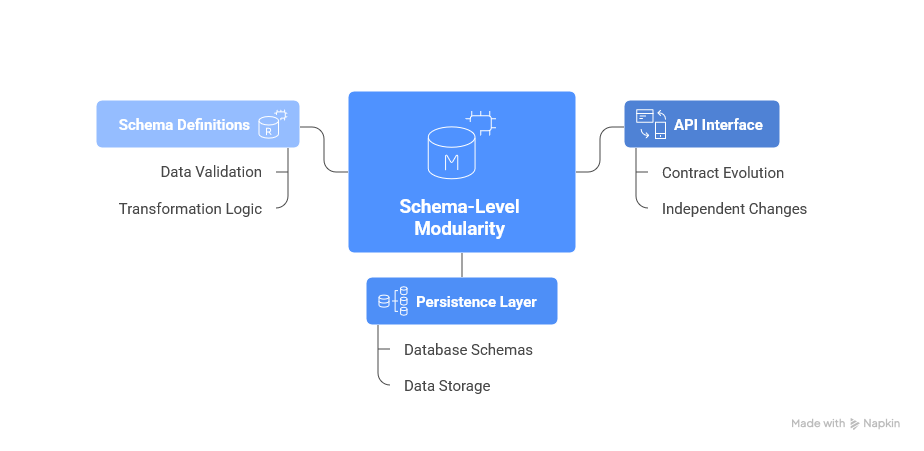
\includegraphics[width=0.9\textwidth]{images/imgs/Schema-Level-Modularity.png}
    \caption{Architecture of Schema-Level Modularity in Data Systems}
    \label{fig:system_architecture}
\end{figure}



\subsection{Separation of Concerns}

Separation of concerns is the principle that different aspects of a system's functionality should be handled by distinct components. This principle reduces complexity by ensuring that each component has a focused responsibility and does not mix unrelated concerns.\hfill \break

Our platform applies separation of concerns through a layered architecture within each service:\hfill \break

\textbf{API Layer:} Handles HTTP request processing, authentication, and response formatting. This layer knows how to receive web requests and send web responses but does not contain business logic or database queries.\hfill \break

\textbf{Service Layer:} Contains business logic and orchestration. This layer implements the rules and workflows of the platform but does not handle HTTP specifics or direct database access.\hfill \break

\textbf{Persistence Layer:} Manages data storage and retrieval. This layer knows how to interact with the database but does not contain business rules or API concerns.\hfill \break

This layering ensures that a change to how data is stored does not require changes to how HTTP requests are processed, and vice versa. Each layer can evolve within its area of responsibility.\hfill \break

\subsection{Extensibility}

Extensibility is the capacity of a system to accommodate new functionality without requiring fundamental structural changes. An extensible system is designed with growth in mind, providing clear points where new capabilities can be added.\hfill \break


Our platform achieves extensibility through several mechanisms:\hfill \break

\textbf{Modular Reconnaissance Engine:} The reconnaissance execution layer is designed as a collection of pluggable modules. Adding support for a new reconnaissance technique, such as a new subdomain source or a different vulnerability database, requires adding a new module rather than modifying existing code.\hfill \break

\textbf{Flexible Data Model:} The persistence schema includes JSON fields that accommodate structured data without requiring schema changes. When a new reconnaissance module produces findings with additional attributes, those attributes can be stored in existing JSON columns.\hfill \break

\textbf{Configuration-Driven Behavior:} Many aspects of system behavior are controlled through configuration rather than code. Enabling or disabling specific data sources, adjusting scanning parameters, or modifying scheduling behavior can be accomplished through configuration changes.\hfill \break

\subsection{Integration-First Design}

Integration-first design prioritizes the ability of a system to work with other systems from the earliest stages of design. Rather than building a standalone system and later adding integration capabilities, integration-first design treats interoperability as a fundamental requirement.\hfill \break

Our platform embodies integration-first design through its API-centric architecture:\hfill \break

\textbf{REST API as Primary Interface:} Every platform capability is exposed through RESTful web service endpoints.\cite{rest_api_best_practices} The API is not an afterthought added to support external tools; it is the primary way that all components, including any user interfaces, interact with platform functionality.\hfill \break

\textbf{Standard Protocols and Formats:} The platform uses widely adopted protocols (HTTP/HTTPS) and data formats (JSON) that virtually any system can work with. No proprietary protocols or formats create barriers to integration.\hfill \break

\textbf{Webhook and Event Patterns:} The architecture supports event-driven patterns where external systems can be notified of platform events, enabling reactive workflows without polling.\hfill \break

\hfill \break These choices were made to maximize interoperability, minimize integration complexity, and future-proof the platform for evolving business needs.

\vspace{1em}
\begin{table}[H]
\centering
\caption{Summary of Integration Design Choices}
\label{tab:integration-choices}
\renewcommand{\arraystretch}{1.3}
\begin{tabular}{|p{3cm}|p{5cm}|p{6.5cm}|}
\hline
\textbf{Design Choice} & \textbf{Alternatives Considered} & \textbf{Rationale} \\
\hline
REST API & GraphQL, gRPC & Broader tooling support, simpler caching, firewall-friendly \\
\hline
JSON format & XML, Protocol Buffers & Human-readable, native JavaScript support, smaller payload than XML \\
\hline
HTTP/HTTPS & Custom TCP protocol & Universal firewall traversal, built-in TLS security, extensive tooling \\
\hline
Webhooks & Polling, WebSockets & Lower resource usage, simpler implementation, real-time delivery \\
\hline
\end{tabular}
\end{table}

\subsection{Asynchronous Processing}

Asynchronous processing decouples the initiation of work from its execution and completion. Rather than forcing callers to wait while operations complete, asynchronous systems accept work requests, queue them for processing, and allow callers to continue with other activities.\hfill \break

Asynchronous processing is essential for our platform because reconnaissance operations are inherently time-consuming. Scanning a large number of targets, querying multiple external services, and performing active reconnaissance can take minutes or hours.\hfill \break

Our platform implements asynchronous processing through a message queue architecture:\hfill \break

\textbf{Job Queue:} When reconnaissance is requested, the request is placed in a queue as a job. The API immediately returns, confirming that the job has been accepted.\hfill \break

\textbf{Worker Processing:} Separate worker processes consume jobs from the queue and execute reconnaissance. Workers operate independently of the API, scaling according to workload.\hfill \break

\textbf{Status Tracking:} Job progress and results are tracked in the database, allowing callers to check status and retrieve results when ready.\hfill \break

\section{Global System Architecture}

Having established our design principles, we now present the overall structure of the platform. This section provides a high-level view before we examine individual components in detail, allowing the reader to understand the system's main organization and its intended operational flow.

\subsection{Architectural Style}

The platform implements a \textbf{distributed microservices architecture}\cite{microservices_arch} with message-based asynchronous communication. This architectural style organizes the system as a collection of loosely coupled services that communicate through well-defined interfaces, promoting modularity, flexibility, and scalability. Each service focuses on a specific business capability, which allows the system to be extended or modified with minimal impact on existing functionality.\hfill \break

The key characteristics of our architecture are:\hfill \break

\textbf{Multiple Deployable Units:} The platform comprises seven distinct services, each packaged as an independent container that can be deployed, started, stopped, and scaled independently. This approach provides the ability to optimize resources and maintain high availability, even under variable loads or during maintenance activities.\hfill \break

\textbf{Service Isolation:} Each service manages its own dependencies and can be updated without affecting other services. A change to the scheduling service, for example, does not require redeploying the API service. This isolation improves fault tolerance and reduces the risk of cascading failures across the platform.\hfill \break

\textbf{Shared Data Store:} While services are independently deployed, they share a common database for persistent data. This shared-data approach provides consistency while allowing service independence. Proper access control and careful schema design ensure that concurrent operations do not interfere with one another, maintaining data integrity across all services.\hfill \break

\textbf{Message-Based Communication:} Services communicate asynchronously through a message queue for operations that do not require immediate responses. This decoupling allows services to operate at their own pace without blocking each other and facilitates reliable event-driven interactions. It also provides a natural mechanism for scaling services independently based on demand.\hfill \break





\begin{figure}[H]
    \centering
    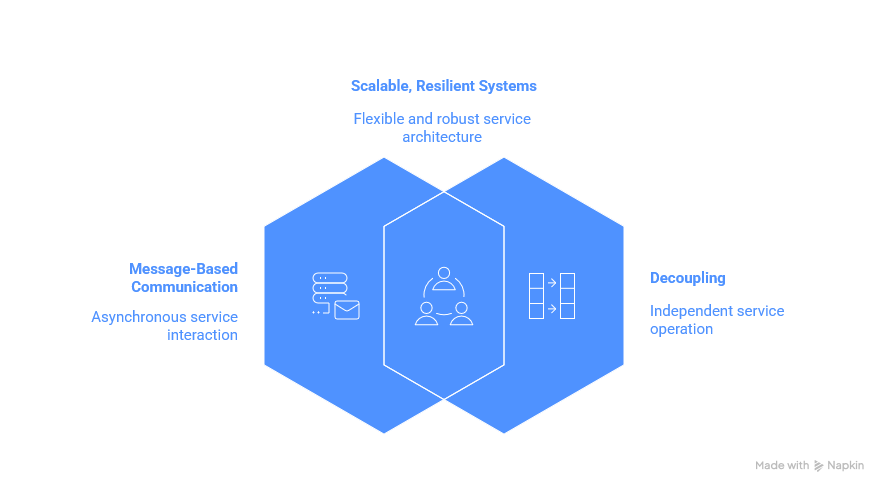
\includegraphics[width=0.9\textwidth]{images/imgs/Message-Driven Decoupled Services.png}
    \caption{Message-Driven Decoupled Services}
    \label{fig:system_architecture}
\end{figure}


\subsection{System Components Overview}

The platform consists of the following major components, each serving a distinct purpose in the overall system:\hfill \break

\begin{table}[H]
\centering
\caption{Summary of Integration Design Choices}
\begin{tabular}{|l|l|l|}
\hline
\textbf{Component} & \textbf{Role} & \textbf{Technology} \\
\hline
Manager API & Primary REST interface for orchestration & FastAPI (Python) \\
\hline
Findings API & Read-only query interface for results & FastAPI (Python) \\
\hline
Engine Worker & Executes reconnaissance jobs & Python worker process \\
\hline
Scheduler Service & Triggers jobs according to schedules & APScheduler (Python) \\
\hline
Database & Persistent storage for all data & PostgreSQL + TimescaleDB \\
\hline
Message Queue & Asynchronous job distribution & Redis \\
\hline
Dashboard & Visualization and monitoring & Grafana \\
\hline
\end{tabular}
\label{tab:components}
\end{table}

The following diagram illustrates how these components interact:\hfill \break

\begin{figure}[H]
    \centering
    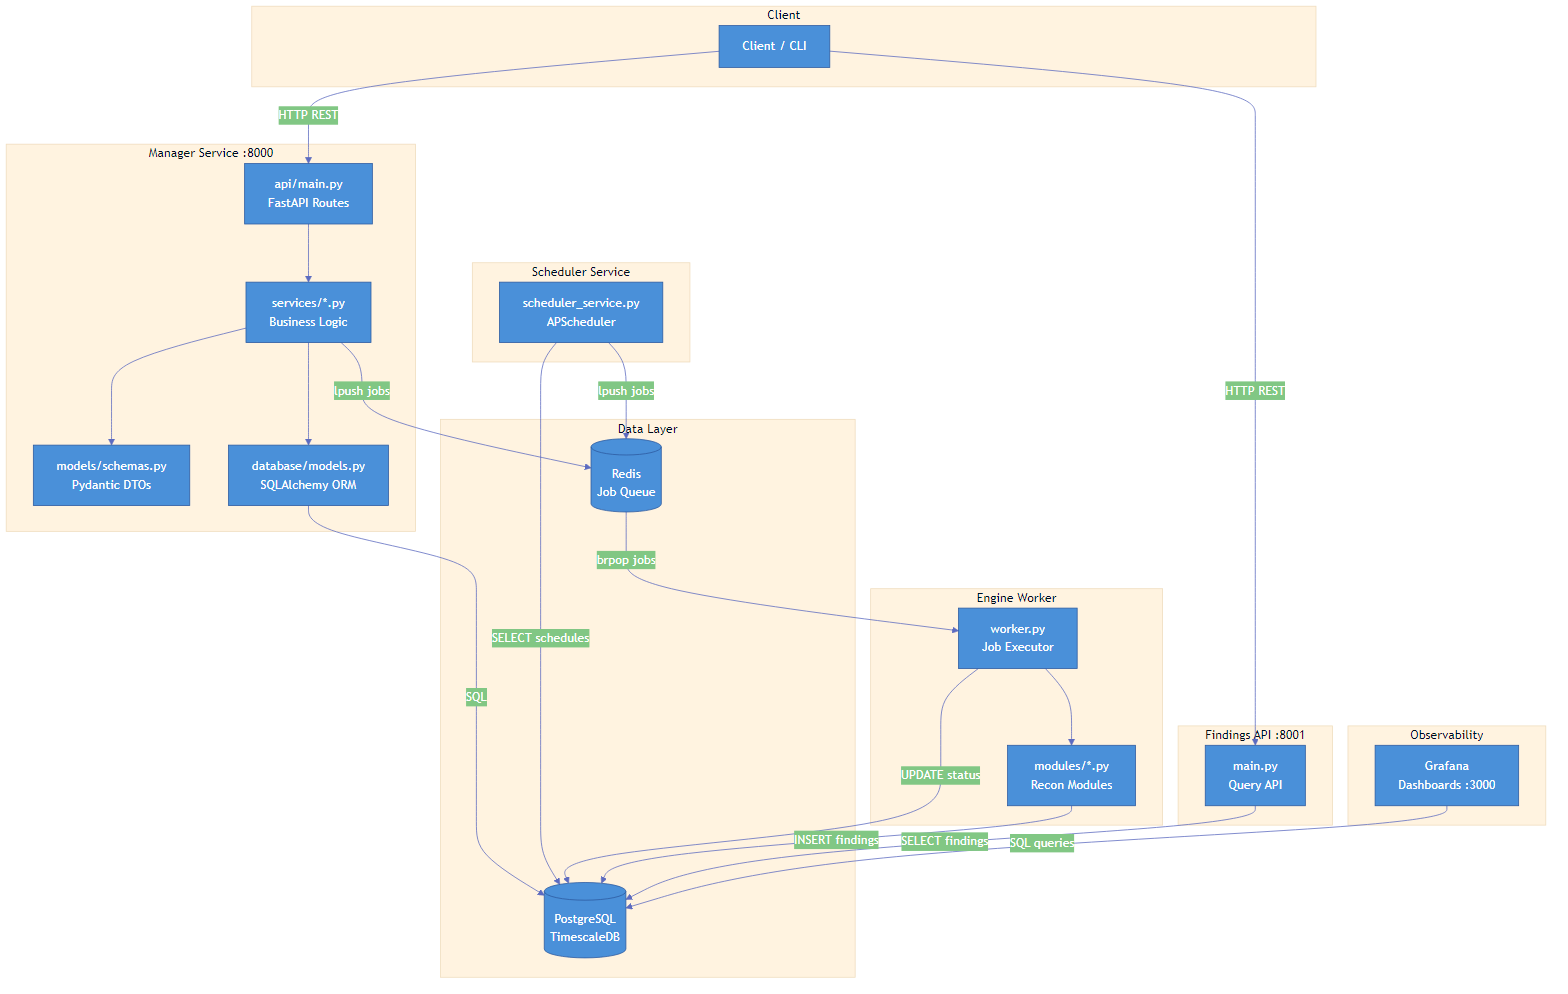
\includegraphics[width=0.9\textwidth]{images/uml/01_system_architecture.png}
    \caption{High-level system architecture showing all seven services and their relationships}
    \label{fig:system_architecture}
\end{figure}

\subsection{Component Interaction Patterns}

Understanding how components interact is as important as understanding what each component does. The platform employs several interaction patterns:\hfill \break

\textbf{Synchronous Request-Response (API Interactions):} When a client sends a request to the Manager API, for example, to create a new reconnaissance target, the interaction follows a synchronous request-response pattern. The client sends an HTTP request, the API processes it, and returns an HTTP response. This pattern is appropriate for operations that complete quickly.\hfill \break

\textbf{Asynchronous Job Processing (Reconnaissance Execution):} When reconnaissance is triggered, either manually through the API or automatically by the scheduler, the work is processed asynchronously. The triggering component places a job message in the Redis queue. The API or scheduler does not wait for reconnaissance to complete; it simply confirms that the job has been queued. The engine worker, operating independently, retrieves jobs from the queue and executes them at its own pace.\hfill \break

\textbf{Polling and Event-Driven Updates (Scheduling):} The scheduler service periodically queries the database for enabled schedules and registers them with its internal scheduling engine. When a schedule's cron expression matches the current time, the scheduler triggers job creation.\hfill \break

\textbf{Direct Database Access (Queries and Persistence):} Multiple services access the shared PostgreSQL database directly for reading and writing data. The Manager API writes configuration data. The engine worker writes findings data. The Findings API reads findings data for query responses. Grafana reads data for dashboard visualizations.\hfill \break

\subsection{High-Level Data Flow}

To understand how the architecture supports the platform's mission, consider the flow of data through a typical reconnaissance operation:\hfill

\begin{enumerate}
\item \textbf{Configuration Entry:} A user configures a reconnaissance scope through the Manager API, specifying targets (domains, IP addresses) and optionally creating a schedule for automated execution.
\item \textbf{Job Triggering:} When reconnaissance is initiated, either by an explicit API call or by a schedule firing, the appropriate service creates a job record in the database and places a job message in the Redis queue.
\item \textbf{Job Execution:} The engine worker retrieves the job message from Redis, queries the database for target details, and begins executing reconnaissance modules.
\item \textbf{External Reconnaissance:} Reconnaissance modules query external services (certificate transparency logs, DNS servers, the Shodan API, etc.) to gather information about the targets.
\item \textbf{Finding Persistence:} As the engine discovers assets and vulnerabilities, it writes findings to the database with timestamps, enabling temporal tracking.
\item \textbf{Status Update:} Upon completion (or failure), the engine updates the job status in the database, recording duration and finding counts.
\item \textbf{Result Access:} Users can query findings through the Findings API or view them through Grafana dashboards.
\end{enumerate}

This flow demonstrates how the architectural components collaborate to deliver the platform's capabilities while maintaining separation of concerns and asynchronous processing.\hfill \break

\section{Component Responsibilities}

We now examine each major component in detail. For each component, we first provide a conceptual explanation suitable for non-technical readers, followed by technical details about its structure and responsibilities.

\subsection{Manager API ,  The Orchestration Gateway}

The Manager API is a FastAPI web application exposing RESTful endpoints for platform management operations. The API follows a layered architecture as illustrated in the following diagram:\hfill \break

\begin{figure}[H]
    \centering
    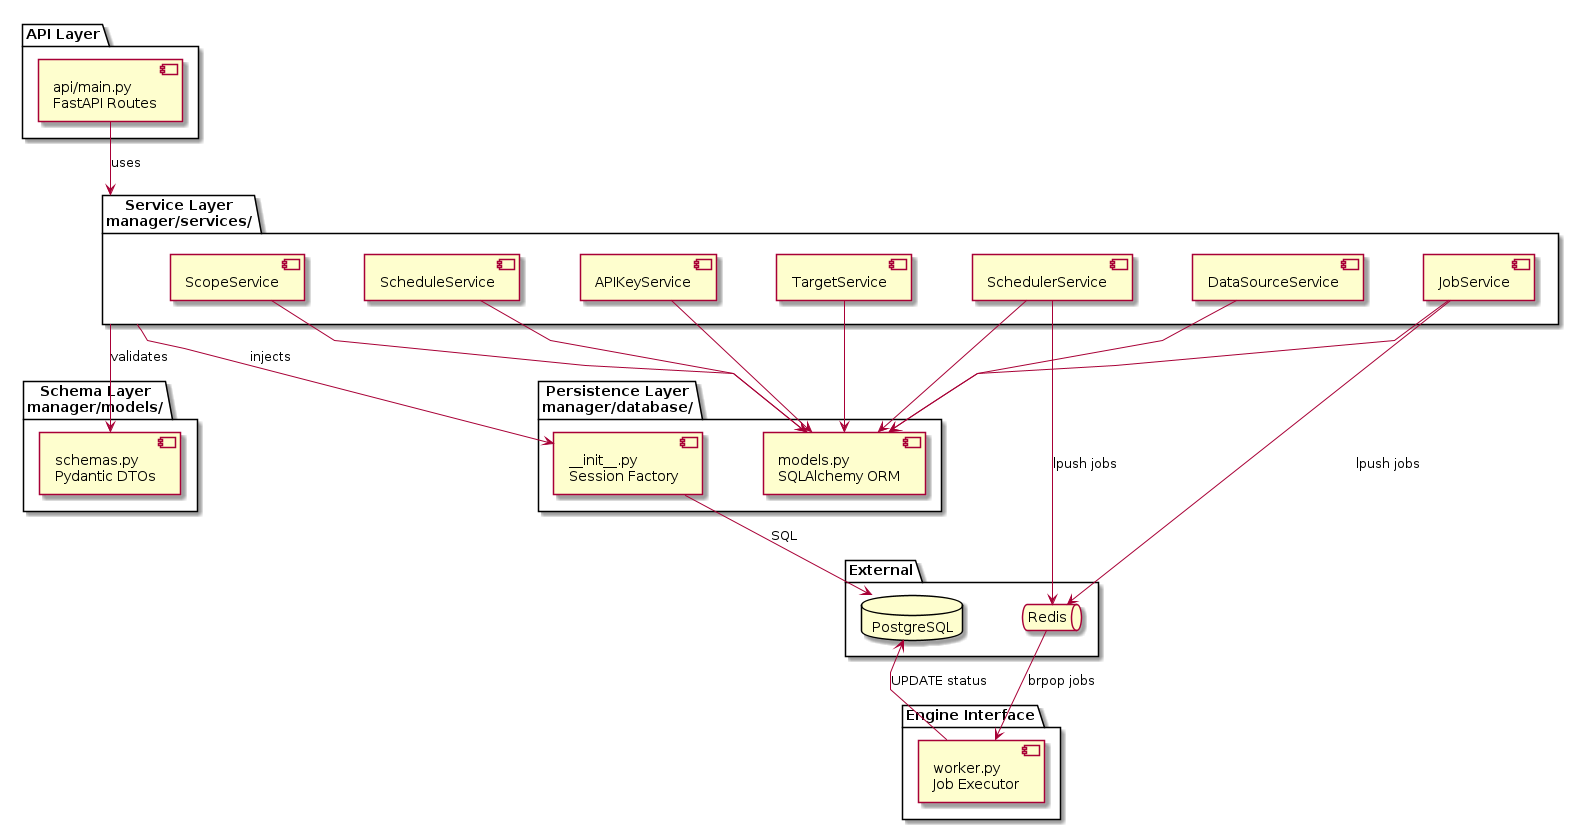
\includegraphics[width=0.85\textwidth]{images/uml/03_service_layer_components.png}
    \caption{Manager API layered architecture showing service layer components}
    \label{fig:service_layer}
\end{figure}

The API layer handles HTTP concerns: routing requests to appropriate handlers, validating request payloads, managing authentication, and formatting responses. Key responsibilities include:\hfill

\begin{itemize}
\item Exposing endpoints for CRUD operations on scopes, targets, schedules, and jobs
\item Validating incoming requests against Pydantic schema definitions
\item Injecting database sessions into service layer components
\item Returning standardized response formats (success/error envelopes, pagination)
\end{itemize}

The API exposes endpoints organized by resource type:\hfill

\begin{table}[H]
\centering
\caption{Manager API endpoints}
\begin{tabular}{|l|l|l|}
\hline
\textbf{Resource} & \textbf{Operations} & \textbf{Purpose} \\
\hline
/api/v1/scopes & Create, Read, Update, Delete & Manage reconnaissance scopes \\
\hline
/api/v1/scopes/\{id\}/targets & Create, Read, Update, Delete & Manage targets within scopes \\
\hline
/api/v1/scopes/\{id\}/schedules & Create, Read, Update, Delete & Manage automated schedules \\
\hline
/api/v1/scopes/\{id\}/jobs & Create (trigger), Read & Initiate and track jobs \\
\hline
/health & Read & Service health verification \\
\hline
\end{tabular}
\label{tab:api_endpoints}
\end{table}

The service layer contains business logic separated from HTTP concerns. Each service class encapsulates operations for a specific domain:\hfill \break

\begin{table}[H]
\centering
\caption{Service layer responsibilities}
\begin{tabular}{|l|l|}
\hline
\textbf{Service} & \textbf{Responsibility} \\
\hline
ScopeService & Scope lifecycle management, configuration validation \\
\hline
TargetService & Target CRUD operations, enable/disable logic \\
\hline
JobService & Job creation, status tracking, queue interaction \\
\hline
ScheduleService & Schedule CRUD, cron expression validation \\
\hline
APIKeyService & External API key management with encryption \\
\hline
DataSourceService & Data source configuration management \\
\hline
\end{tabular}
\label{tab:services}
\end{table}

\subsection{Findings API ,  The Query Interface}

The Findings API is a separate FastAPI application focused exclusively on read operations against the findings data. This service:\hfill

\begin{itemize}
\item Provides endpoints for querying findings by scope, job, time range, and finding type
\item Supports aggregation queries (counts, summaries, statistics)
\item Enables export functionality for findings data
\item Implements pagination for large result sets
\end{itemize}

Key query endpoints include:\hfill \break

\begin{table}[H]
\centering
\caption{Findings API endpoints}
\begin{tabular}{|l|l|}
\hline
\textbf{Endpoint} & \textbf{Purpose} \\
\hline
/api/v1/scopes/\{id\}/findings & Retrieve findings for a scope with filtering \\
\hline
/api/v1/scopes/\{id\}/summary & Aggregated statistics for a scope \\
\hline
/api/v1/scopes/\{id\}/subdomains & Subdomain-specific findings \\
\hline
/api/v1/scopes/\{id\}/dns & DNS record findings \\
\hline
/api/v1/jobs/\{id\}/findings & Findings from a specific job \\
\hline
/api/v1/summary & Platform-wide summary statistics \\
\hline
\end{tabular}
\label{tab:findings_endpoints}
\end{table}

The Findings API connects directly to the PostgreSQL database with read-only access. Its queries leverage TimescaleDB's time-series optimization for efficient filtering by time ranges.\hfill \break

\subsection{Execution Engine ,  The Reconnaissance Worker}

The engine is a Python worker process that consumes job messages from Redis and orchestrates reconnaissance execution. The engine architecture comprises several layers as shown in the following diagram:\hfill \break

\begin{figure}[H]
    \centering
    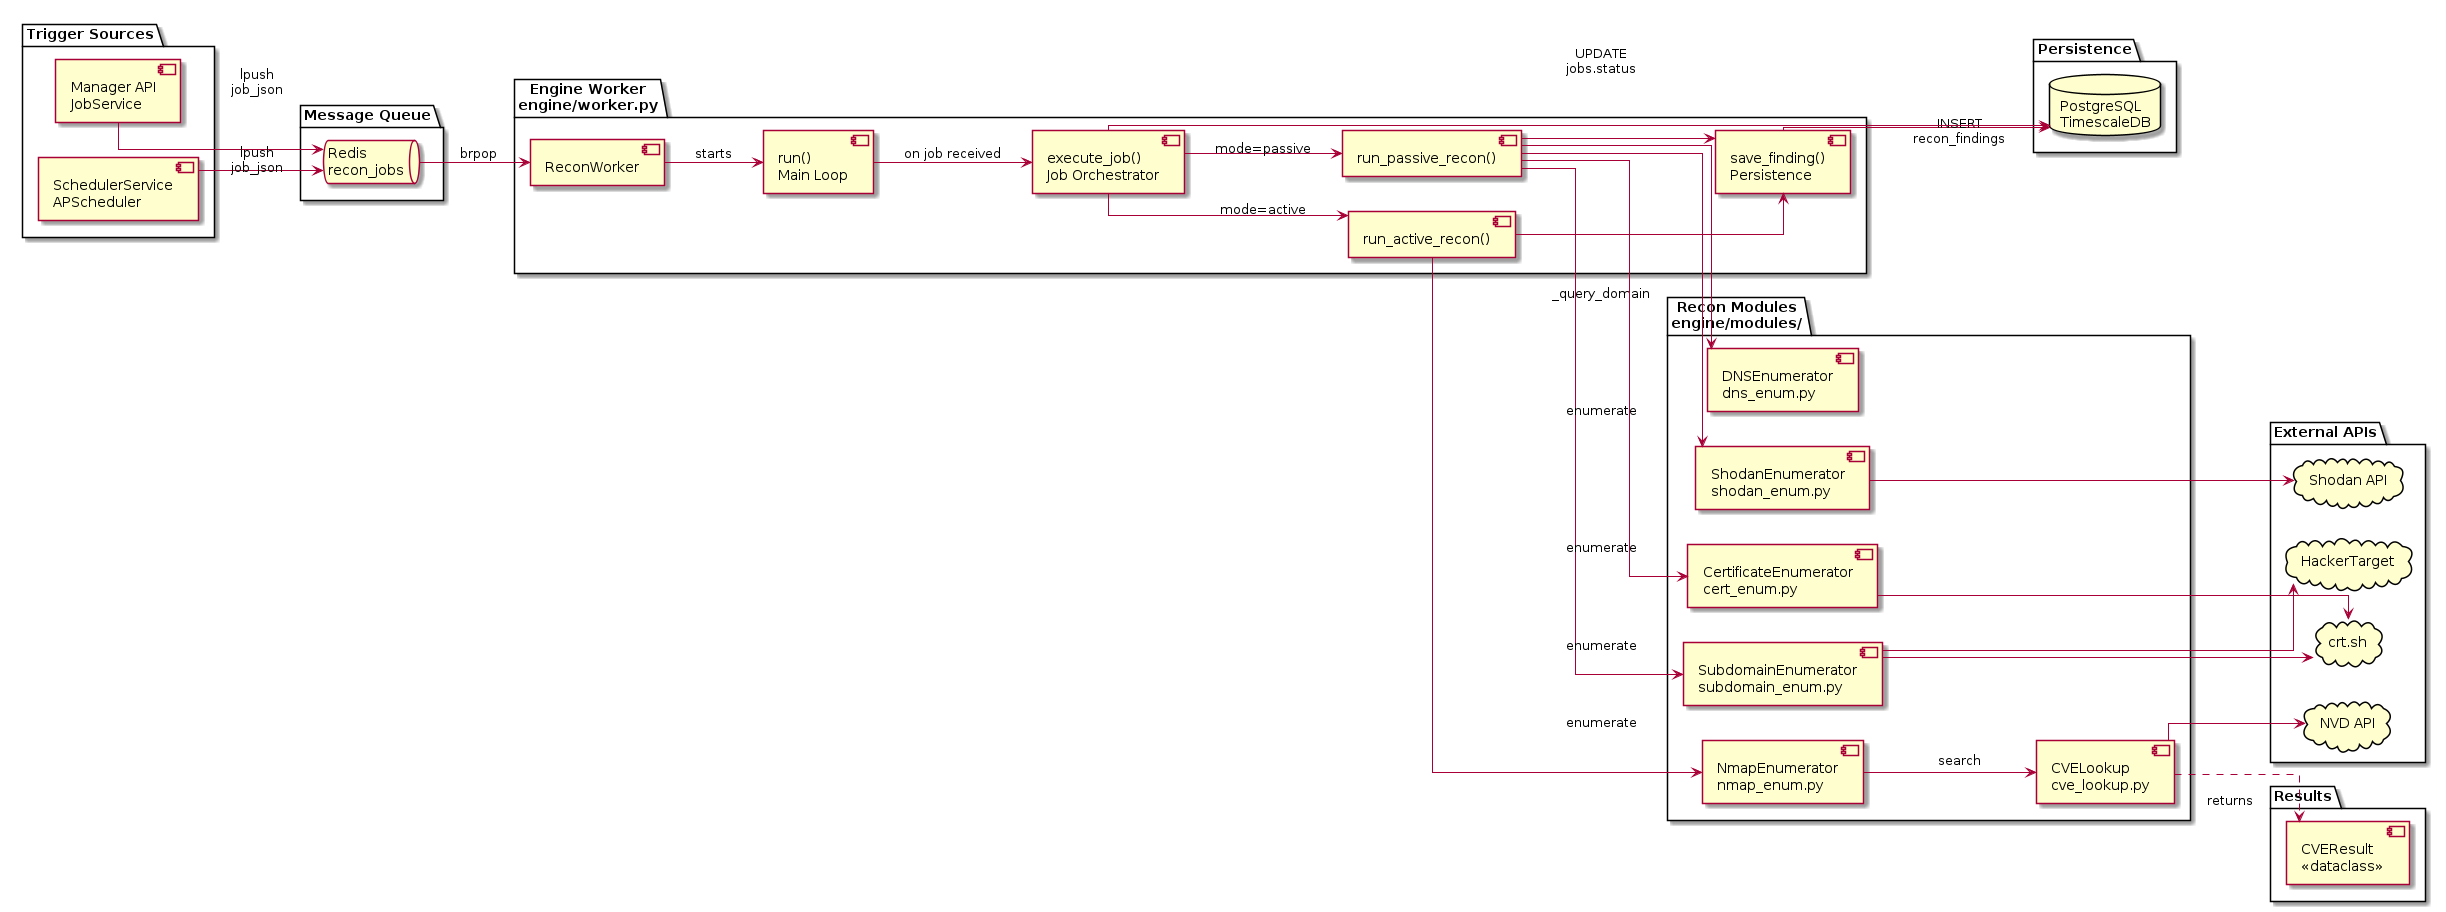
\includegraphics[width=0.9\textwidth]{images/uml/04_engine_execution_layer.png}
    \caption{Engine Worker architecture showing reconnaissance modules}
    \label{fig:engine_architecture}
\end{figure}

The worker process implements a continuous loop:\hfill \break

\begin{enumerate}
\item Block waiting for a job message from Redis (brpop operation)
\item Parse the job payload to extract scope ID, mode, and configuration
\item Update job status to "running" in the database
\item Fetch target details from the database
\item Execute reconnaissance based on the specified mode
\item Persist findings to the database
\item Update job status to "completed" with statistics
\item Return to step 1
\end{enumerate}

The actual reconnaissance logic is encapsulated in discrete modules:\hfill \break

\begin{table}[H]
\centering
\caption{Reconnaissance modules}
\begin{tabular}{|l|l|l|}
\hline
\textbf{Module} & \textbf{Class} & \textbf{Capability} \\
\hline
subdomain\_enum & SubdomainEnumerator & Passive subdomain discovery from 12+ sources \\
\hline
dns\_enum & DNSEnumerator & DNS record resolution (A, AAAA, MX, TXT, NS) \\
\hline
cert\_enum & CertificateEnumerator & Certificate transparency \cite{cert_transparency} log queries via crt.sh \cite{crtsh_api} \\
\hline
shodan\_enum & ShodanEnumerator & Shodan \cite{shodan_api} API for host intelligence \\
\hline
nmap\_enum & NmapEnumerator & Nmap \cite{nmap_docs} port scanning and service detection \\
\hline
cve\_lookup & CVELookup & NVD \cite{nvd_api} API for vulnerability correlation \\
\hline
\end{tabular}
\label{tab:recon_modules}
\end{table}

The engine supports two reconnaissance modes:\hfill \break

\textbf{Passive Mode:} Executes only modules that gather information without directly interacting with target systems. This includes subdomain enumeration from public sources, certificate transparency queries, and Shodan lookups.\hfill \break

\textbf{Active Mode:} Extends passive reconnaissance with modules that directly interact with target systems. This adds Nmap port scanning and service detection.\hfill \break

\subsection{Scheduler Service ,  The Automation Controller}

The scheduler service uses APScheduler, a Python scheduling library that supports cron-style schedule expressions. The service operates as follows:\hfill \break

\textbf{Schedule Discovery:} The scheduler periodically queries the database for enabled schedules. Each schedule record contains a scope identifier, a cron expression, a reconnaissance mode, and enable/disable status.\hfill \break

\textbf{Cron Expression Processing:} Cron expressions define when jobs should execute using a standard format specifying minute, hour, day of month, month, and day of week. For example:
\begin{itemize}
\item \texttt{0 2 * * *} ,  Every day at 2:00 AM
\item \texttt{0 */6 * * *} ,  Every 6 hours
\item \texttt{0 0 * * 0} ,  Every Sunday at midnight
\end{itemize}

\textbf{Job Triggering:} When a schedule fires, the scheduler creates a job record in the database with triggered\_by='scheduler', pushes a job message to the Redis queue, and updates the schedule's last\_run timestamp.\hfill \break

\subsection{Persistence Layer ,  The Data Foundation}

The persistence layer centers on PostgreSQL \cite{postgresql_docs} enhanced with TimescaleDB \cite{timescaledb_docs} for time-series capabilities. The data model comprises several entity categories as illustrated in the following diagram:\hfill \break

\begin{figure}[H]
    \centering
    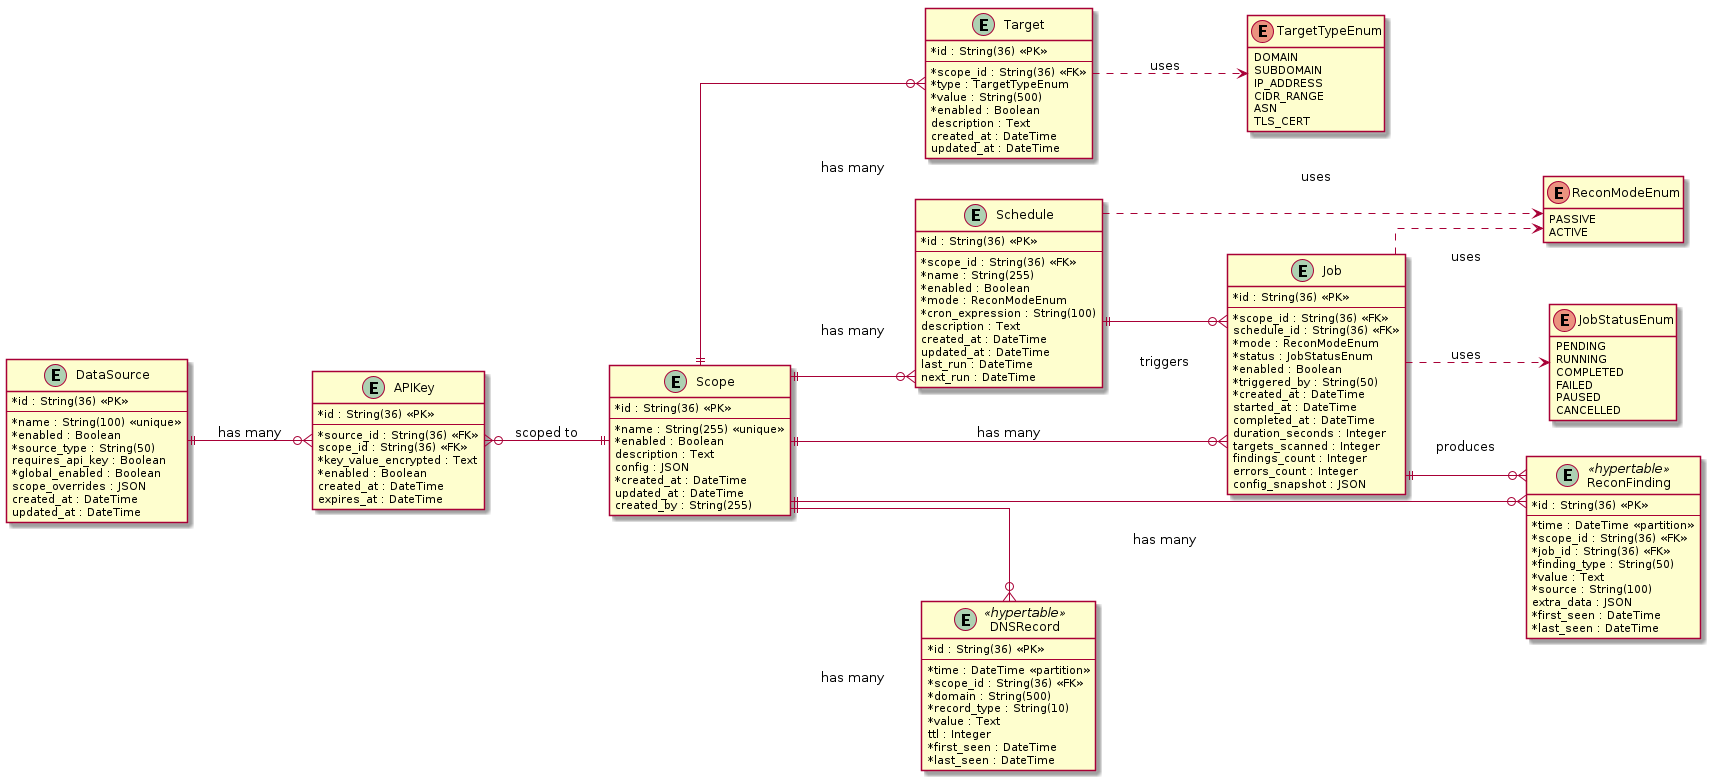
\includegraphics[width=0.9\textwidth]{images/uml/01_domain_persistence_model.png}
    \caption{Domain persistence model showing entities and relationships}
    \label{fig:persistence_model}
\end{figure}

\textbf{Configuration Entities:} These entities represent the platform's configuration state:\hfill \break

\begin{table}[H]
\centering
\caption{Configuration entities}
\begin{tabular}{|l|l|l|}
\hline
\textbf{Entity} & \textbf{Purpose} & \textbf{Key Attributes} \\
\hline
Scope & Organizational grouping & name, enabled, config (JSON) \\
\hline
Target & Reconnaissance target & scope\_id, type, value, enabled \\
\hline
Schedule & Automated execution config & scope\_id, cron\_expression, mode \\
\hline
DataSource & External service config & name, source\_type, enabled \\
\hline
APIKey & Encrypted credentials & source\_id, key\_value\_encrypted \\
\hline
\end{tabular}
\label{tab:config_entities}
\end{table}

\textbf{Operational Entities:} These entities track platform operations:\hfill \break

\begin{table}[H]
\centering
\caption{Operational entities}
\begin{tabular}{|l|l|l|}
\hline
\textbf{Entity} & \textbf{Purpose} & \textbf{Key Attributes} \\
\hline
Job & Execution record & scope\_id, mode, status, findings\_count \\
\hline
\end{tabular}
\label{tab:operational_entities}
\end{table}

\textbf{Time-Series Entities (Hypertables):} These entities store reconnaissance findings with temporal indexing:\hfill \break

\begin{table}[H]
\centering
\caption{Time-series entities}
\begin{tabular}{|l|l|l|}
\hline
\textbf{Entity} & \textbf{Purpose} & \textbf{Key Attributes} \\
\hline
ReconFinding & General findings storage & time, scope\_id, finding\_type, value \\
\hline
DNSRecord & DNS-specific findings & time, domain, record\_type, value, ttl \\
\hline
\end{tabular}
\label{tab:timeseries_entities}
\end{table}

TimescaleDB automatically partitions hypertables by time, enabling efficient queries over time ranges and automatic data retention management.\hfill \break

\subsection{Message Queue ,  The Asynchronous Backbone}

The platform uses Redis \cite{redis_docs} as its message queue, leveraging Redis's list data structures and blocking operations: \hfill 

\begin{table}[H]
\centering
\caption{Queue operations}
\begin{tabular}{|l|l|l|}
\hline
\textbf{Operation} & \textbf{Used By} & \textbf{Purpose} \\
\hline
lpush & Manager API, Scheduler & Add job to queue \\
\hline
brpop & Engine Worker & Retrieve job from queue (blocking) \\
\hline
\end{tabular}
\label{tab:queue_ops}
\end{table}

The brpop (blocking right pop) operation is particularly important, it allows the engine worker to wait efficiently for new jobs without busy-polling, consuming minimal resources when idle.\hfill \break

The queue architecture provides several benefits:
\begin{itemize}
\item \textbf{Decoupling:} API and engine operate independently
\item \textbf{Buffering:} Jobs accumulate during high load periods
\item \textbf{Scalability:} Multiple engine workers can consume from the same queue
\item \textbf{Resilience:} Jobs persist in Redis if the engine restarts
\end{itemize}

\subsection{Observability Layer ,  Visualization and Monitoring}

The platform integrates Grafana \cite{grafana_docs} as its visualization layer. Grafana connects directly to the PostgreSQL \cite{postgresql_docs} database, executing queries against the findings tables to populate dashboard panels.\hfill 

The Grafana deployment includes:
\begin{itemize}
\item \textbf{Provisioned Data Source:} Automatic configuration connecting Grafana to PostgreSQL
\item \textbf{Provisioned Dashboards:} Pre-built attack surface dashboard deployed automatically
\item \textbf{Query-Based Panels:} Each panel executes SQL queries against the findings data
\end{itemize}

The pre-configured dashboard provides:\hfill \break

\begin{table}[H]
\centering
\caption{Dashboard panels}
\begin{tabular}{|l|l|}
\hline
\textbf{Panel Type} & \textbf{Information Displayed} \\
\hline
Stat panels & Total subdomains, open ports, CVE counts \\
\hline
Tables & Target lists, job history, finding details \\
\hline
Time series & Trends over time for key metrics \\
\hline
Pie charts & Distribution of findings by type or severity \\
\hline
\end{tabular}
\label{tab:dashboard_panels}
\end{table}

\section{Communication Boundaries and Data Ownership}

Understanding what data each component owns and how components communicate is essential for maintaining architectural integrity. This section maps these boundaries explicitly.

\subsection{Data Ownership Matrix}

Each database table has a clear owner, the component responsible for writing to that table:\hfill \break

\begin{table}[H]
\centering
\caption{Data ownership matrix}
\begin{tabular}{|l|l|l|}
\hline
\textbf{Table} & \textbf{Write Owner} & \textbf{Readers} \\
\hline
scopes & Manager API & Scheduler, Engine, Findings API, Grafana \\
\hline
targets & Manager API & Engine \\
\hline
schedules & Manager API & Scheduler \\
\hline
jobs & Manager API, Engine & Findings API, Grafana \\
\hline
recon\_findings & Engine & Findings API, Grafana \\
\hline
dns\_records & Engine & Findings API, Grafana \\
\hline
api\_keys & Manager API & Engine \\
\hline
data\_sources & Manager API & Engine \\
\hline
\end{tabular}
\label{tab:data_ownership}
\end{table}

Note that jobs has two write owners: the Manager API creates job records when jobs are triggered, while the Engine updates status and statistics as jobs execute.\hfill \break

\subsection{Communication Patterns}

\begin{table}[H]
\centering
\caption{Communication patterns}
\begin{tabular}{|l|l|l|l|}
\hline
\textbf{From} & \textbf{To} & \textbf{Mechanism} & \textbf{Purpose} \\
\hline
Client & Manager API & HTTP REST & Configuration, job triggering \\
\hline
Client & Findings API & HTTP REST & Query results \\
\hline
Manager API & PostgreSQL & SQL & Persist configuration \\
\hline
Manager API & Redis & Queue push & Dispatch jobs \\
\hline
Scheduler & PostgreSQL & SQL & Read schedules, create jobs \\
\hline
Scheduler & Redis & Queue push & Dispatch scheduled jobs \\
\hline
Engine & Redis & Queue pop & Receive job assignments \\
\hline
Engine & PostgreSQL & SQL & Read config, write findings \\
\hline
Engine & External APIs & HTTP & Reconnaissance data gathering \\
\hline
Findings API & PostgreSQL & SQL & Read findings \\
\hline
Grafana & PostgreSQL & SQL & Read data for visualization \\
\hline
\end{tabular}
\label{tab:communication}
\end{table}

\subsection{Boundary Enforcement}

Maintaining clean boundaries requires discipline. The following rules govern component interactions:\hfill \break

\textbf{Manager API Boundaries:} Handles all configuration writes. Never executes reconnaissance logic. Delegates job execution to engine via queue.\hfill \break

\textbf{Engine Boundaries:} Never exposes HTTP endpoints. Never modifies configuration entities. Owns all finding persistence.\hfill \break

\textbf{Findings API Boundaries:} Strictly read-only. Never writes to any table. Never triggers jobs or modifies configuration.\hfill \break

\textbf{Scheduler Boundaries:} Only creates jobs at scheduled times. Never executes reconnaissance. Never modifies schedules (only reads them).\hfill \break

\section{Technology Selection Rationale}

The technologies comprising our platform were selected deliberately based on requirements analysis. This section explains the rationale for key technology choices.

\subsection{Python as the Implementation Language}

Python was selected as the primary implementation language for several reasons:\hfill

\begin{itemize}
\item \textbf{Rich ecosystem for security tooling:} Libraries exist for DNS resolution, HTTP requests, API interactions, and integration with tools like Nmap \cite{nmap_docs}
\item \textbf{FastAPI \cite{fastapi_docs} framework availability:} Modern, high-performance API framework with automatic documentation
\item \textbf{Rapid development:} Dynamic typing and extensive standard library accelerate development
\item \textbf{Community familiarity:} Python is widely known in the security community
\end{itemize}

\subsection{FastAPI for API Services}

FastAPI provides: \hfill

\begin{itemize}
\item \textbf{Automatic OpenAPI documentation:} API documentation generated from code
\item \textbf{Pydantic \cite{pydantic_docs} integration:} Declarative request/response validation
\item \textbf{Async support:} Efficient handling of concurrent requests
\item \textbf{Modern Python features:} Type hints, dependency injection
\end{itemize}

\subsection{PostgreSQL with TimescaleDB}

The database selection addresses both relational and time-series requirements:\hfill

\begin{itemize}
\item \textbf{PostgreSQL \cite{postgresql_docs}:} Mature, reliable relational database with excellent tooling
\item \textbf{TimescaleDB \cite{timescaledb_docs} extension:} Purpose-built time-series capabilities on PostgreSQL foundation
\item \textbf{Unified storage:} Single database engine for all data, simplifying operations
\end{itemize}

\subsection{Redis for Message Queue}

Redis provides simple, reliable queueing:\hfill

\begin{itemize}
\item \textbf{List operations:} Native support for queue patterns
\item \textbf{Blocking operations:} Efficient worker waiting
\item \textbf{Proven reliability:} Widely deployed in production systems
\item \textbf{Low operational overhead:} Simple to deploy and manage
\end{itemize}

\subsection{Docker for Deployment}

Container-based deployment provides:

\begin{itemize}
\item \textbf{Environment consistency:} Same behavior across development and production
\item \textbf{Isolation:} Services run in separate containers
\item \textbf{Orchestration:} Docker \cite{docker_docs} Compose \cite{docker_compose_docs} defines complete deployment
\item \textbf{Dependency management:} Each container includes its dependencies
\end{itemize}

\section*{Conclusion}
\addcontentsline{toc}{section}{Conclusion}

In this chapter, we have presented the architectural foundation of our threat exposure management platform. We began by establishing the design principles that guided our decisions: modularity, separation of concerns, extensibility, integration-first design, and asynchronous processing. These principles ensure that the platform can evolve to meet changing requirements while maintaining structural integrity.\hfill \break

We then examined the global system architecture, a distributed microservices design comprising seven distinct components: the Manager API for orchestration, the Findings API for queries, the Engine Worker for reconnaissance execution, the Scheduler Service for automation, PostgreSQL with TimescaleDB for persistence, Redis for message queueing, and Grafana for visualization.\hfill \break

For each component, we explained both its conceptual role, what it does in terms accessible to non-technical readers, and its technical structure, how it accomplishes its responsibilities. We mapped the boundaries between components, clarifying data ownership and communication patterns that maintain architectural discipline.\hfill \break

The technology selections underlying our architecture reflect deliberate choices aligned with our requirements: Python for its security tooling ecosystem, FastAPI for modern API development, PostgreSQL with TimescaleDB for unified relational and time-series storage, Redis for simple reliable queueing, and Docker for consistent deployment.\hfill \break

In the next chapter, we will move from architecture to implementation, examining how these components were realized in code. We will walk through the implementation of key modules, trace the execution of primary use cases, and explore the data models and validation logic that ensure system integrity.\hfill \break

%%%%%%%%%%%%%%%%%%%%%%%%%%%%%%%%%%%%%%%%%%%%%%%%%%%%%%%%%%%%%%%%%%%%%%%%%%%%%%%%%
%%%%%%%%%%%%%%%%%%%%%%%%%%%%%%%%%%%%%%%%%%%%%%%%%%%%%%%%%%%%%%%%%%%%%%%%%%%%%%%%%
%%%%%%%%%%%%%%%%%%%%%%%%%%%%%%%%%%%%%%%%%%%%%%%%%%%%%%%%%%%%%%%%%%%%%%%%%%%%%%%%%

\chapter{Implementation and Realization}
\thispagestyle{plain}
\section*{Introduction}
\addcontentsline{toc}{section}{Introduction}
Having established the architectural foundation of our threat exposure management platform in the previous chapter, we now turn to implementation, the process of translating architectural designs into working code. This chapter bridges the gap between conceptual design and operational reality.\hfill \break

Implementation is where architectural intentions meet technical constraints. A well-designed architecture provides a blueprint, but the quality of implementation determines whether the system actually delivers on that blueprint's promises. Poor implementation can undermine excellent architecture, while thoughtful implementation can compensate for architectural limitations.\hfill \break

We will examine implementation through several lenses. First, we will explore the project structure and how code is organized within each service. Then, we will trace the implementation of major use cases, showing how user requests flow through the system. We will examine the data models that define our domain, the API layer that exposes platform capabilities, and the reconnaissance modules that perform the actual work of asset discovery. Throughout, we will include code excerpts and diagrams that illustrate key implementation patterns.\cite{plantuml_docs}\hfill \break

This chapter assumes familiarity with basic programming concepts. Where we use technical terminology, we will provide explanations accessible to readers with general technical backgrounds.

\section{Project Structure and Organization}

Before examining specific implementations, it is helpful to understand how the codebase is organized. A well-structured project enables developers to locate code quickly, understand component boundaries, and make changes with confidence.

\subsection{Repository Layout}

The platform is organized as a monorepo, a single repository containing all services. This approach simplifies dependency management and enables atomic changes across services when needed. The top-level structure separates services, shared components, and infrastructure configuration:\hfill \break

\begin{verbatim}
threat-exposure-platform/
├── manager_api/           # Manager API service
├── findings_api/          # Findings API service  
├── engine/                # Reconnaissance engine
├── scheduler/             # Scheduler service
├── shared/                # Shared utilities and models
├── grafana/               # Dashboard configurations
├── docker/                # Dockerfiles and compose files
\end{verbatim}

Each service follows a consistent internal structure that reflects the layered architecture described in Chapter 2. The Manager API, as the most complex service, exemplifies this structure:\hfill \break

\begin{verbatim}
manager_api/
├── api/
│   ├── routes/            # API endpoint definitions
│   │   ├── scopes.py
│   │   ├── targets.py
│   │   ├── schedules.py
│   │   └── jobs.py
│   ├── schemas/           # Request/response models
│   │   ├── scope_schemas.py
│   │   ├── target_schemas.py
│   │   └── common.py
│   └── dependencies.py    # Dependency injection
├── services/              # Business logic layer
│   ├── scope_service.py
│   ├── target_service.py
│   ├── job_service.py
│   └── schedule_service.py
├── models/                # SQLAlchemy ORM models
│   ├── scope.py
│   ├── target.py
│   └── base.py
├── core/                  # Configuration and utilities
│   ├── config.py
│   ├── database.py
│   └── security.py
├── main.py                # Application entry point
└── requirements.txt       # Python dependencies
\end{verbatim}

This structure enforces separation of concerns through directory organization. A developer modifying how HTTP requests are handled knows to look in \texttt{api/routes/}. A developer changing business logic looks in \texttt{services/}. Database schema changes occur in \texttt{models/}.\hfill \break

\subsection{Shared Components}

The \texttt{shared/} directory contains code used by multiple services, preventing duplication and ensuring consistency:\hfill \break

\begin{table}[H]
\centering
\begin{tabular}{|l|l|}
\hline
\textbf{Component} & \textbf{Purpose} \\
\hline
shared/models/ & SQLAlchemy model definitions used by multiple services \\
\hline
shared/schemas/ & Pydantic schemas for cross-service data validation \\
\hline
shared/utils/ & Common utilities (logging, encryption, formatting) \\
\hline
shared/constants.py & Enumeration values and constants \\
\hline
shared/exceptions.py & Custom exception classes \\
\hline
\end{tabular}
\caption{Shared components}
\label{tab:shared_components}
\end{table}

By centralizing model definitions, we ensure that all services interpret database entities identically. When a schema changes, the change propagates to all services through the shared module.\hfill \break

\section{Data Models Implementation}

Data models form the foundation of any information system. They define what data the system stores, how data elements relate to each other, and what constraints govern data validity. Our implementation uses SQLAlchemy, a Python Object-Relational Mapping (ORM) library that allows us to define database structures as Python classes.

\subsection{Object-Relational Mapping Concepts}

For readers unfamiliar with ORM, a brief explanation is helpful. Databases store data in tables with rows and columns. Object-oriented programming languages organize code around objects with attributes and methods. An ORM bridges these paradigms, allowing developers to work with database records as if they were Python objects.\hfill \break

When we define a SQLAlchemy model class, we are simultaneously defining:
\begin{itemize}
\item A Python class with attributes
\item A database table with columns
\item Rules for converting between the two representations
\end{itemize}

\subsection{Core Entity Models}

The \texttt{Scope} model represents the primary organizational unit in our platform. A scope groups related reconnaissance targets and serves as the context for jobs, schedules, and findings. Key design decisions for this model include:

\begin{itemize}
\item \textbf{UUID Primary Keys:} UUIDs support distributed systems and prevent information leakage about record counts
\item \textbf{JSONB Configuration:} Flexible storage of structured configuration data without schema changes
\item \textbf{Cascade Deletion:} Automatic cleanup of associated targets, schedules, and jobs when a scope is deleted
\item \textbf{Timestamps:} Automatic tracking of creation and modification times
\end{itemize}

The \texttt{Target} model represents individual reconnaissance targets within a scope. Targets are constrained to predefined types (domain, IP address, CIDR range, or URL) through database enumerations.\hfill \break

\subsection{Job and Schedule Models}

The \texttt{Job} model tracks reconnaissance execution with a defined lifecycle: PENDING → RUNNING → (COMPLETED | FAILED). Each job records its execution mode, trigger source (API or scheduler), timing information, findings count, and any error messages. This comprehensive tracking enables operational monitoring and debugging.\hfill \break

The \texttt{Schedule} model defines automated reconnaissance schedules using cron expressions for flexible timing configuration. Schedules track their last execution time and can be independently enabled or disabled without deletion.\hfill \break

\subsection{Time-Series Finding Models}

Reconnaissance findings require special handling due to their time-series nature. We use TimescaleDB hypertables for efficient storage and querying of temporal data. The \texttt{ReconFinding} model uses a composite primary key of timestamp and UUID, enabling TimescaleDB's automatic partitioning while maintaining uniqueness.\hfill \break

Key design features include:
\begin{itemize}
\item \textbf{Automatic Partitioning:} TimescaleDB partitions data into 7-day chunks for efficient time-range queries
\item \textbf{Flexible Attributes:} A JSONB column stores finding-specific details that vary by finding type
\item \textbf{Optimized Indexing:} Indexes on scope and time enable efficient filtering by scope and time range
\end{itemize}

\section{API Layer Implementation}

The API layer translates HTTP requests into service operations and formats results as HTTP responses. This section examines how we implement RESTful endpoints using FastAPI.

\subsection{FastAPI Application Structure}

FastAPI applications are built from routers, modular collections of related endpoints. Our Manager API assembles routers for each resource type (scopes, targets, schedules, jobs), each prefixed with \texttt{/api/v1/} to enable API versioning. The application automatically generates OpenAPI documentation at \texttt{/api/docs}.\hfill \break

A health check endpoint at \texttt{/health} reports service status for container orchestration and monitoring systems.\hfill \break

\subsection{Request Validation with Pydantic Schemas}

Pydantic schemas define the structure and validation rules for request and response data. When a request arrives, FastAPI automatically validates the payload against the schema, returning detailed error messages for invalid input.\hfill \break

Our schemas implement:
\begin{itemize}
\item \textbf{Type Constraints:} Fields are typed with enumerations (e.g., target types: domain, IP, CIDR, URL)
\item \textbf{Value Validation:} Custom validators ensure values match expected formats (valid domain names, valid IP addresses)
\item \textbf{Response Transformation:} Response schemas convert database models to API-friendly formats with proper serialization
\end{itemize}

\subsection{Endpoint Implementation Pattern}

Each endpoint follows a consistent pattern: receive request, validate input, delegate to service layer, return formatted response. This separation ensures that HTTP concerns remain in the API layer while business logic resides in services.\hfill \break

The pattern includes:
\begin{itemize}
\item \textbf{Dependency Injection:} Database sessions are injected automatically and closed when requests complete
\item \textbf{Error Handling:} HTTP exceptions with appropriate status codes (404 Not Found, 409 Conflict, etc.)
\item \textbf{Response Formatting:} Automatic serialization of response models to JSON
\end{itemize}

\subsection{Response Formatting}

API responses follow consistent patterns for both success and error cases. Paginated responses include metadata about the total result set (total count, current page, page size, total pages), preventing overwhelming responses when querying large datasets.\hfill \break

Error responses include the error type, detailed message, HTTP status code, and timestamp for debugging and logging purposes.\hfill \break

\section{Service Layer Implementation}

The service layer contains business logic independent of HTTP concerns. Services coordinate operations, enforce business rules, and orchestrate interactions between multiple components.

\subsection{Service Class Pattern}

Each service class encapsulates operations for a specific domain entity. Services receive a database session at construction, enabling transaction management. This pattern provides:

\begin{itemize}
\item \textbf{CRUD Operations:} Standard create, read, update, delete operations for each entity type
\item \textbf{Query Methods:} Filtered retrieval by various criteria (ID, name, scope, etc.)
\item \textbf{Transaction Control:} Explicit commit and refresh operations for data consistency
\item \textbf{Business Rules:} Validation and enforcement of domain-specific rules
\end{itemize}

\subsection{Job Service and Queue Integration}

The Job Service demonstrates integration between the service layer and the message queue. When creating a job, the service performs a dual-write pattern:

\begin{enumerate}
\item Create and persist the job record in the database with PENDING status
\item Publish a job message to the Redis queue containing job ID, scope ID, and mode
\end{enumerate}

This pattern requires careful consideration for production systems, if the database write succeeds but the queue publish fails, the job will exist but never execute.\hfill \break

\section{Reconnaissance Engine Implementation}

The reconnaissance engine is the platform's workhorse, executing the actual discovery operations. This section examines how the engine processes jobs and coordinates reconnaissance modules.

\subsection{Worker Process Architecture}

The engine runs as a continuous worker process, waiting for jobs from the Redis queue. The worker uses Redis's blocking pop operation (\texttt{brpop}), which blocks efficiently until a message arrives, consuming no CPU while waiting.\hfill \break

When a job message arrives, the executor handles all reconnaissance logic. If job execution fails, the worker continues processing subsequent jobs.\hfill \break

\subsection{Reconnaissance Executor}

The executor coordinates job execution, managing status updates and delegating to specialized modules. The following diagram illustrates the execution flow:\hfill \break

\begin{figure}[H]
    \centering
    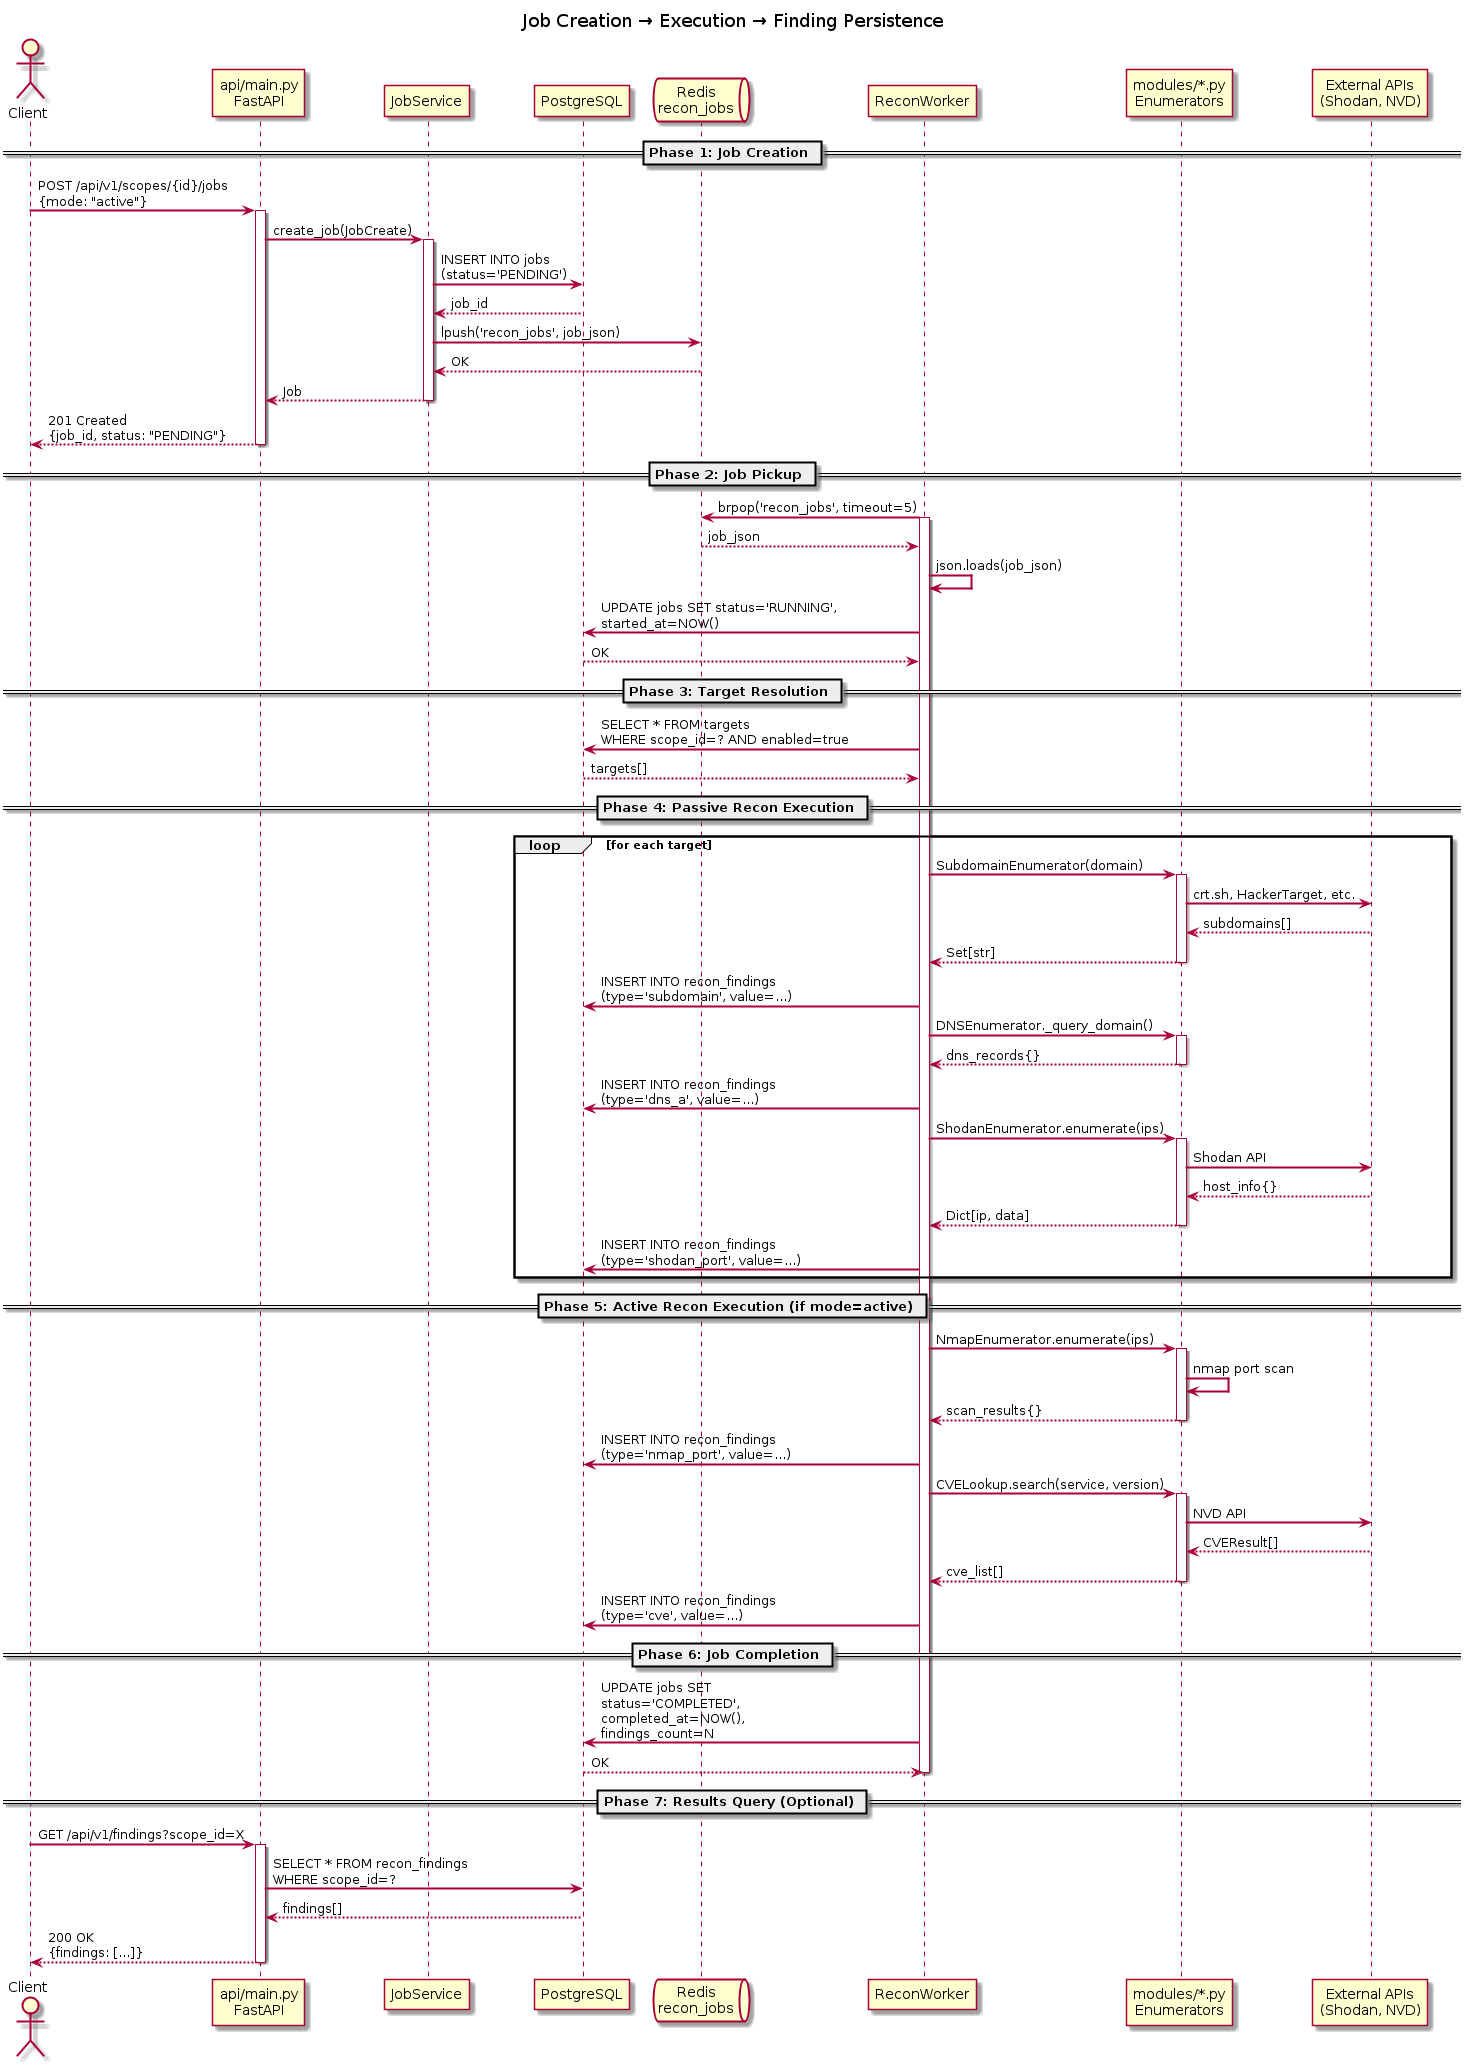
\includegraphics[width=1\textwidth, height=1.1\textwidth]{images/uml/05_recon_execution_sequence.png}
    \caption{Reconnaissance execution sequence diagram}
    \label{fig:recon_sequence}
\end{figure}

The executor workflow consists of:\hfill \break
\begin{enumerate}
\item Update job status to RUNNING and record start time
\item Load enabled targets for the scope from the database
\item Execute passive reconnaissance modules (subdomain enumeration, DNS resolution, Shodan queries, CVE lookup)
\item If active mode is requested, additionally execute active modules (Nmap port scanning)
\item Persist all findings to the database with timestamps
\item Update job status to COMPLETED with findings count
\end{enumerate}

The modular approach enables different reconnaissance capabilities to be enabled or disabled independently, and new modules can be added without modifying the executor logic.\hfill \break

\subsection{Module Interface Pattern}

All reconnaissance modules implement a common interface, enabling the executor to treat them uniformly. Each module provides:

\begin{itemize}
\item \textbf{Name:} A unique identifier for logging and configuration
\item \textbf{Description:} Human-readable explanation of the module's purpose
\item \textbf{Execute Method:} Takes targets and database session, returns a list of findings
\end{itemize}

Each finding is a structured dictionary containing the finding type (subdomain, port, CVE, etc.), data source identifier, primary value, and additional attributes. This standardized interface enables new reconnaissance capabilities to be added by implementing the interface without modifying the executor.\hfill \break

\subsection{Subdomain Enumeration Module}

The subdomain enumeration module queries multiple public sources to discover subdomains associated with target domains. It aggregates results from over twelve data sources including:

\begin{itemize}
\item \textbf{Certificate Transparency Logs:} crt.sh provides access to SSL certificate transparency data
\item \textbf{Security Intelligence APIs:} HackerTarget, ThreatCrowd, AlienVault OTX
\item \textbf{Web Archives:} URLScan.io and similar services
\end{itemize}

The module deduplicates results as it queries each source. Error handling ensures that one source's failure does not prevent results from other sources, resilience is prioritized over completeness from any single source.\hfill \break

\subsection{DNS Enumeration Module}

The DNS enumeration module resolves DNS records for discovered assets. It queries for multiple record types including A, AAAA, MX, TXT, NS, and CNAME records.\hfill \break

For each domain target and discovered subdomain, the module:\hfill \break
\begin{enumerate}
\item Attempts resolution for each record type
\item Records successful resolutions with TTL values
\item Gracefully handles NXDOMAIN (non-existent domain) and NoAnswer conditions
\item Continues processing other domains if individual lookups fail
\end{enumerate}

This comprehensive DNS data provides valuable infrastructure intelligence, revealing mail servers, name servers, and IP address mappings.\hfill \break

\subsection{Shodan Integration Module}

The Shodan module queries the Shodan API for host intelligence. When configured with a valid API key (stored encrypted in the database), the module:

\begin{itemize}
\item Queries Shodan for IP target information including exposed services
\item Extracts port, protocol, product, version, and banner information for each service
\item Identifies known vulnerabilities associated with discovered hosts
\item Gracefully handles API errors and rate limits
\end{itemize}

If Shodan is not configured (no API key), the module returns empty results without causing job failure.\hfill \break

\section{Scheduler Service Implementation}

The scheduler service enables automated reconnaissance execution according to configured schedules.

\subsection{APScheduler Integration}

The scheduler uses APScheduler,\cite{apscheduler_docs} a Python scheduling library that supports cron-style expressions. The service operates through:\hfill \break

\textbf{Schedule Discovery:} The scheduler periodically (every 5 minutes) queries the database for enabled schedules and synchronizes its internal job registry.\hfill \break

\textbf{Cron Expression Processing:} Standard cron format defines when jobs execute using APScheduler.\cite{apscheduler_docs} Examples:
\begin{itemize}
\item \texttt{0 2 * * *} ,  Every day at 2:00 AM
\item \texttt{0 */6 * * *} ,  Every 6 hours
\item \texttt{0 0 * * 0} ,  Every Sunday at midnight
\end{itemize}

\textbf{Job Triggering:} When a schedule fires, the scheduler creates a job record with \hfill \break \texttt{triggered\_by='scheduler'}, pushes a job message to Redis, and updates the schedule's \texttt{last\_run} timestamp.
The scheduler maintains synchronization between database schedules and APScheduler jobs, allowing schedule changes through the API to take effect without restarting the scheduler service.\hfill \break

\section{Use Case Walkthroughs}

To demonstrate how components work together, we trace the execution of a representative use case through the system.

\subsection{Use Case: Manual Reconnaissance Trigger}

This use case follows a user manually triggering reconnaissance through the API:\hfill \break

\begin{figure}[H]
    \centering
    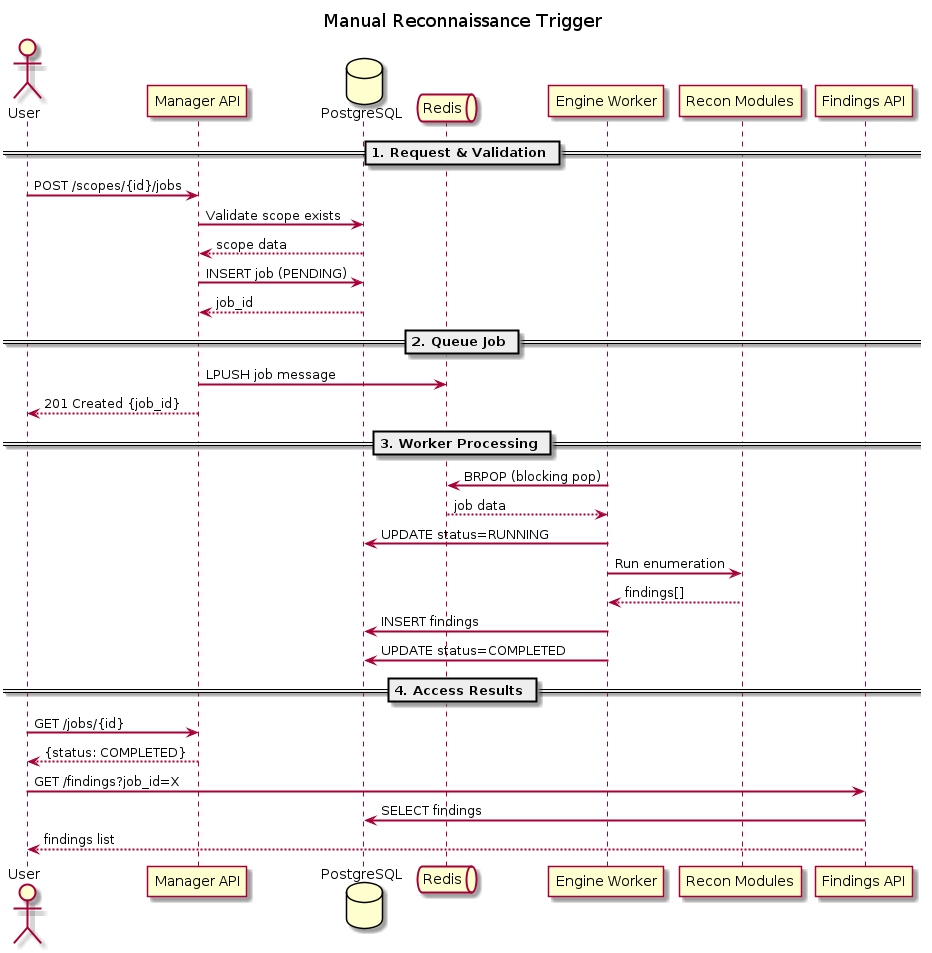
\includegraphics[width=0.9\textwidth, height=0.7\textwidth]{images/uml/06_manual_trigger_sequence.png}
    \caption{Sequence diagram illustrating the manual reconnaissance execution workflow}
    \label{fig:manual_trigger}
\end{figure}

The workflow proceeds as follows:\hfill \break

\begin{enumerate}
\item \textbf{API Request:} User sends POST to \texttt{/api/v1/scopes/\{scope\_id\}/jobs} with reconnaissance mode
\item \textbf{Validation:} API validates the request, verifies scope exists and is enabled
\item \textbf{Job Creation:} Service creates job record (PENDING status) and publishes to Redis queue
\item \textbf{Response:} API returns 201 Created with job details
\item \textbf{Engine Processing:} Worker receives job, updates to RUNNING, executes reconnaissance modules, persists findings
\item \textbf{Completion:} Job status updated to COMPLETED with findings count
\item \textbf{Result Access:} User queries job status and findings via API or views in Grafana dashboard
\end{enumerate}

Scheduled reconnaissance follows the same pattern, with the scheduler service triggering jobs at configured times instead of API requests.\hfill \break

\section{Error Handling Strategy}

Robust error handling is essential for production systems. The platform implements error handling at multiple levels:\hfill \break

\textbf{API Layer:} Structured error responses with appropriate HTTP status codes. Validation errors return 422 with detailed field-level messages. Not found conditions return 404. Internal errors are logged with full stack traces while returning sanitized 500 responses to clients.\hfill \break

\textbf{Job-Level Isolation:} Each job's failure is isolated, one job's exception does not affect other jobs. Failed jobs are marked with FAILED status and error messages are recorded for debugging.\hfill \break

\textbf{Module-Level Isolation:} Within reconnaissance execution, individual module failures do not prevent other modules from executing. If the Shodan API is temporarily unavailable, the job still completes with findings from other sources.\hfill \break

This layered isolation ensures the platform degrades gracefully under adverse conditions, maintaining availability even when individual components encounter errors.\hfill \break

\section*{Conclusion}
\addcontentsline{toc}{section}{Conclusion}

In this chapter, we have examined the implementation of our threat exposure management platform, translating the architectural designs from Chapter 2 into working code. We began with project structure, showing how the codebase is organized to support maintainability and clear separation of concerns.\hfill \break

We explored data models implemented with SQLAlchemy, demonstrating how Python classes map to database tables while enforcing relationships and constraints. The API layer implementation showed how FastAPI enables declarative endpoint definitions with automatic validation through Pydantic schemas.\hfill \break

The service layer implementation revealed how business logic is encapsulated separately from HTTP and database concerns. The reconnaissance engine implementation demonstrated the modular execution architecture, where specialized modules perform different types of discovery while the executor coordinates their execution.\hfill \break

Through use case walkthroughs, we traced complete request flows through the system, showing how components collaborate to deliver functionality. Error handling patterns demonstrated the resilience strategies that ensure the platform degrades gracefully under adverse conditions.\hfill \break

The code excerpts and diagrams presented in this chapter provide insight into implementation decisions and patterns. While we could not include every detail of a substantial codebase, the examples illustrate the core implementation approaches that define the platform's character.\hfill \break

In the next chapter, we will move from implementation to deployment, examining how the platform is containerized, orchestrated, and operated in practice. We will explore the Docker Compose configuration, environment management, and operational procedures that transform code into a running system.\hfill \break

%%%%%%%%%%%%%%%%%%%%%%%%%%%%%%%%%%%%%%%%%%%%%%%%%%%%%%%%%%%%%%%%%%%%%%%%%%%%%%%%%
%%%%%%%%%%%%%%%%%%%%%%%%%%%%%%%%%%%%%%%%%%%%%%%%%%%%%%%%%%%%%%%%%%%%%%%%%%%%%%%%%
%%%%%%%%%%%%%%%%%%%%%%%%%%%%%%%%%%%%%%%%%%%%%%%%%%%%%%%%%%%%%%%%%%%%%%%%%%%%%%%%%

\chapter{Deployment, Execution, and Integration}
\thispagestyle{plain}
\section*{Introduction}
\addcontentsline{toc}{section}{Introduction}
Software exists to be used, and software that cannot be deployed reliably provides no value regardless of how elegantly it is implemented. This chapter addresses the critical transition from code to running system, the deployment, execution, and integration practices that transform our threat exposure management platform from a collection of source files into an operational service.\hfill \break

Deployment encompasses more than simply starting applications. It includes environment configuration, dependency management, service orchestration, health monitoring, and the operational procedures that keep systems running over time. For a distributed platform like ours, deployment complexity is substantial: multiple services must be configured consistently, databases must be initialized with proper schemas, services must discover and communicate with each other, and the entire ensemble must be manageable as a coherent unit.\hfill \break

We will examine containerization with Docker, orchestration with Docker Compose, environment configuration management, database initialization, and the operational lifecycle of the deployed platform. We will also explore integration patterns that enable the platform to work with external systems and dashboards that provide operational visibility.

\section{Containerization Strategy}

Containerization packages applications with their dependencies into portable, isolated units that run consistently across environments. Our platform uses Docker containers to achieve deployment consistency and simplify operations.

\subsection{Service Dockerfiles}

Each platform service has a Dockerfile specifying how to build its container image. Key design decisions include:

\begin{itemize}
\item \textbf{Base Image:} Python 3.11-slim for minimal attack surface and image size
\item \textbf{Layer Optimization:} Dependencies installed before code copy for efficient caching
\item \textbf{Security:} Non-root user execution inside containers
\item \textbf{Health Checks:} Built-in health endpoints for orchestration monitoring
\end{itemize}

The Engine Worker Dockerfile includes additional system dependencies (Nmap,\cite{nmap_docs} dnsutils) required for active reconnaissance capabilities.\hfill \break

\section{Service Orchestration with Docker Compose}

Docker Compose orchestrates multi-container applications, defining services, networks, and volumes in a declarative configuration.

\subsection{Compose Architecture}

Our Docker Compose\cite{docker_compose_docs} configuration defines the complete platform stack with the following services:\hfill \break

\begin{table}[H]
\centering
\caption{Docker Compose services}
\begin{tabular}{|l|l|l|}
\hline
\textbf{Service} & \textbf{Image/Build} & \textbf{Port} \\
\hline
postgres & timescale/timescaledb:latest-pg15 & 5432 \\
\hline
redis & redis:7-alpine & 6379 \\
\hline
manager-api & Built from ./manager\_api & 8000 \\
\hline
findings-api & Built from ./findings\_api & 8001 \\
\hline
engine & Built from ./engine & N/A (worker) \\
\hline
scheduler & Built from ./scheduler & N/A (background) \\
\hline
grafana & grafana/grafana:latest & 3000 \\
\hline
\end{tabular}
\label{tab:compose_services}
\end{table}

The platform is started with a single command:
\begin{verbatim}
docker compose up -d
\end{verbatim}

\subsection{Service Dependencies and Configuration}

Docker Compose manages service startup order through health-based dependencies. Application services (APIs, engine, scheduler) wait for infrastructure services (PostgreSQL, Redis) to report healthy status before starting. This prevents race conditions where services attempt to connect to databases not yet ready.\hfill \break

All services connect to a shared bridge network, referencing each other by container name. Docker volumes persist database files, Redis data, and Grafana configurations across container restarts.\hfill \break

\section{Environment Configuration}

Production systems require careful configuration management. Sensitive values like database credentials must not be hardcoded in source files.

\subsection{Environment Variables}

The platform uses environment variables for configuration, following the twelve-factor app methodology. A \texttt{.env} file provides environment-specific values for database credentials, Redis connection, Grafana credentials, API secrets, and external API keys (Shodan, NVD).\hfill \break

The \texttt{.env} file is excluded from version control via \texttt{.gitignore}. A template file (\texttt{.env.example}) documents required variables without sensitive values.\hfill \break

Within services, Pydantic settings classes load and validate environment variables, ensuring required configuration is present before the application starts.\hfill \break

\section{Database Initialization}

Before the platform can operate, the database must be initialized with the correct schema and extensions.

\subsection{Migration Strategy}

Alembic, a database migration tool for SQLAlchemy, \cite{sqlalchemy_docs} manages schema changes. Migrations are versioned scripts that can be applied sequentially to bring a database to the current schema state. The initial migration enables TimescaleDB \cite{timescaledb_docs} and UUID extensions, creates configuration tables (scopes, targets, schedules), operational tables (jobs), and time-series hypertables for findings.\hfill 

TimescaleDB's \texttt{create\_hypertable} function converts the findings table to a hypertable with 7-day chunk intervals for efficient time-range queries.\hfill \break

\section{Deployment Procedures}

\subsection{Initial Deployment}

First-time deployment follows these steps:\hfill \break

\begin{enumerate}
\item Clone repository and configure \texttt{.env} file
\item Build images: \texttt{docker compose build}
\item Start infrastructure: \texttt{docker compose up -d postgres redis}
\item Run database migrations
\item Start all services: \texttt{docker compose up -d}
\item Verify health endpoints and logs
\end{enumerate}

\begin{figure}[H]
    \centering
    \includegraphics[width=1\textwidth]{images/screenshots/docker_compose_up.png}
    \caption{Docker Compose deployment output showing all services starting}
    \label{fig:docker_compose}
\end{figure}

\subsection{Service Updates and Scaling}

Service updates use rolling restarts with \texttt{docker compose up -d --no-deps <service>} to avoid unnecessary dependent service restarts. The engine worker can be horizontally scaled using \texttt{docker compose up -d --scale engine=3} to handle increased job load.\hfill \break

\section{Platform Operation and Monitoring}

\subsection{Health and Log Management}

Each service exposes health check endpoints reporting service status. Docker's built-in health checks automatically restart containers that fail repeatedly.\hfill \break

Service logs are accessible via \texttt{docker compose logs} with options for following real-time output, filtering by service, and limiting output lines. For production deployments, logs should be aggregated to a centralized logging system.\hfill \break

\subsection{Grafana Dashboard Integration}

Grafana provides operational visibility through pre-configured dashboards automatically loaded at startup.\hfill \break

\begin{figure}[H]
    \centering
    \includegraphics[width=1\textwidth]{images/screenshots/grafana_dashboard_overview.png}
    \caption{Grafana dashboard showing attack surface overview}
    \label{fig:grafana_overview}
\end{figure}

The dashboard displays total discovered subdomains, ports, and vulnerabilities; job execution history and success rates; finding trends over time; and per-scope breakdowns. Grafana connects directly to PostgreSQL, executing queries against the findings tables.\hfill \break

\section{API Integration Patterns}

The platform's API-centric design enables integration with external systems through several patterns:\hfill \break

\textbf{Webhook Notifications:} External systems can receive notifications of platform events (job completion, new findings) through configured webhook URLs.\hfill \break

\textbf{SIEM Integration:} Findings can be exported in formats compatible with Security Information and Event Management systems, such as Common Event Format (CEF) for syslog integration.\hfill \break

\textbf{Programmatic Access:} External systems integrate through the REST API for scope management, target configuration, job triggering, and findings retrieval.\hfill \break

\section{Execution Demonstration}

To illustrate the platform in operation, we present a complete execution walkthrough from configuration through results visualization.

\subsection{Creating a Reconnaissance Scope}

Using the Manager API, we create a scope and add targets:\hfill \break

\begin{figure}[H]
    \centering
    \includegraphics[width=1\textwidth]{images/screenshots/api_create_scope.png}
    \caption{Creating a reconnaissance scope via API}
    \label{fig:create_scope}
\end{figure}

\begin{verbatim}
# Create scope
curl -X POST http://localhost:8000/api/v1/scopes \
  -H "Content-Type: application/json" \
  -d '{"name": "Example Corp", "description": "Demo scope"}'

# Add domain target
curl -X POST http://localhost:8000/api/v1/scopes/{scope_id}/targets \
  -H "Content-Type: application/json" \
  -d '{"target_type": "domain", "value": "example.com"}'
\end{verbatim}

\subsection{Triggering and Monitoring Reconnaissance}

With the scope configured, we trigger passive reconnaissance and monitor progress:\hfill \break

\begin{verbatim}
# Trigger passive reconnaissance
curl -X POST http://localhost:8000/api/v1/scopes/{scope_id}/jobs \
  -H "Content-Type: application/json" \
  -d '{"mode": "passive"}'

# Check job status
curl http://localhost:8000/api/v1/scopes/{scope_id}/jobs/{job_id}
\end{verbatim}

\subsection{Querying and Visualizing Results}

The Findings API provides access to discovered assets:\hfill \break

\begin{figure}[H]
    \centering
    \includegraphics[width=1\textwidth]{images/screenshots/api_findings_response.png}
    \caption{API response showing discovered subdomains}
    \label{fig:findings_response}
\end{figure}

\section{Observed Benefits and Operational Results}

Following the deployment and execution of the platform, several tangible benefits were observed across security, operational, and managerial dimensions. This section presents the practical impact of the system based on real execution results rather than theoretical expectations.

\subsection{Impact on Security Teams}

\textbf{Improved Attack Surface Visibility:}  
During execution, the platform successfully identified external-facing assets using multiple discovery techniques in parallel. By aggregating results from different reconnaissance modules, security teams obtained a consolidated and consistent view of the organization’s external exposure, reducing blind spots commonly caused by reliance on a single discovery method.\hfill \break

\textbf{Actionable Risk Prioritization:}  
Discovered assets were automatically correlated with vulnerability and exposure data. This correlation enabled security teams to focus on high-risk assets first, transforming raw reconnaissance data into prioritized security actions.\hfill \break

\textbf{Reduced Manual Effort:}  
Automated scheduling and execution eliminated the need for manual scan initiation. As a result, teams were able to dedicate more time to analysis and remediation rather than repetitive reconnaissance tasks.\hfill \break

\begin{figure}[H]
    \centering
    \includegraphics[width=01\textwidth]{images/screenshots/grafana_findings_detail.png}
    \caption{Grafana dashboard showing reconnaissance findings breakdown}
    \label{fig:grafana_findings}
\end{figure}


\subsection{Results for Organizational Leadership}

\textbf{High-Level Risk Visibility:}  
The platform provided aggregated metrics and dashboards that summarized the organization’s external attack surface. These views allowed non-technical stakeholders to assess security posture without requiring detailed technical knowledge.\hfill \break

\textbf{Trend Analysis Over Time:}  
By retaining historical execution data, the platform enabled temporal analysis of attack surface evolution. Leadership could observe whether exposure levels were increasing or decreasing across multiple execution cycles, providing insight into the effectiveness of security initiatives.\hfill \break

\textbf{Data-Driven Decision Support:}  
Quantitative measurements, such as asset counts and vulnerability distribution, offered concrete evidence to support security investment decisions. Observed trends helped justify resource allocation and long-term security planning.\hfill \break


\begin{figure}[H]
    \centering
    \includegraphics[width=1\textwidth]{images/screenshots/cve.png}
    \caption{High-Level Visualization of External Exposure and Vulnerability Distribution
}
    \label{fig:High-Level Visualization of External Exposur}
\end{figure}

\subsection{Operational and Technical Outcomes}

\textbf{Execution Transparency:}  
Throughout deployment and operation, all reconnaissance activities were fully observable. Operations teams could clearly identify which modules were executed, their scheduling frequency, and the scope of assessed assets.\hfill \break

\textbf{Adaptability and Customization:}  
The modular architecture allowed teams to enable, disable, or extend specific components based on operational requirements. This flexibility ensured that the platform could adapt to different environments without structural changes.\hfill \break

\textbf{Scalable Execution Performance:}  
The distributed microservices architecture proved effective in scaling reconnaissance workloads. Individual services could be scaled independently to accommodate increased discovery or analysis demand without impacting overall system stability.\hfill \break

\begin{figure}[H]
    \centering
    \includegraphics[width=01\textwidth]{images/screenshots/image.png}
    \caption{Technical Dashboard Illustrating Reconnaissance Execution and Module Activity
}
    \label{fig:Technical Dashboard Illustrating Reconnaissance Execution}
\end{figure}



\section*{Conclusion}
\addcontentsline{toc}{section}{Conclusion}

In this chapter, we have examined the deployment, execution, and integration aspects of our threat exposure management platform. We began with containerization, Docker Compose orchestration, environment configuration, and operational procedures. Database initialization and migration procedures ensure consistent schema changes. Integration patterns enable REST APIs, webhooks, and SIEM-compatible exports for external system integration.\hfill \break

In practical testing, the platform successfully demonstrates the feasibility of continuous threat exposure management. The deployment completes within minutes with all services initializing correctly. The modular architecture proved effective with modules executing independently and gracefully degrading when data sources are unavailable. DNS enumeration successfully resolved thousands of DNS records, Shodan integration correctly identified open ports and services, and CVE correlation successfully mapped software versions to vulnerabilities. The API layer handles concurrent requests with acceptable response times, and Grafana dashboards provide meaningful operational visibility with comprehensive statistics and detailed findings.\hfill \break

These results validate our architectural approach. The separation of concerns into specialized services combined with asynchronous job processing enables a system responsive to user requests while capable of long-running reconnaissance operations. The platform successfully addresses the core challenge: providing continuous visibility into digital attack surfaces without requiring constant manual intervention. This chapter completes our technical examination. We have progressed from problem statement through architecture, implementation, and deployment into a deployable, operable system capable of continuous threat exposure assessment.\hfill \break



%%%%%%%%%%%%%%%%%%%%%%%%%%%%%%%%%%%%%%%%%%%%%%%%%%%%%%%%%%%%%%%%%%%%%%%%%%%%%%%%%%%%%%%%%%
%%%%%%%%%%%%%%%%%%%%%%%%%%%%%%%%%%%%%%%%%%%%%%%%%%%%%%%%%%%%%%%%%%%%%%%%%%%%%%%%%%%%%%%%%%
%%%%%%%%%%%%%%%%%%%%%%%%%%%%%%%%%%%%%%%%%%%%%%%%%%%%%%%%%%%%%%%%%%%%%%%%%%%%%%%%%%%%%%%%%%

\newpage
\thispagestyle{plain}
\addcontentsline{toc}{chapter}{General Conclusion}
\section*{General Conclusion}
\label{chapter:General Conclusion}

This project set out to address a fundamental challenge in modern cybersecurity: the need for continuous, comprehensive visibility into an organization's digital attack surface. As organizations increasingly rely on distributed digital infrastructure, the traditional approach of periodic security assessments has become insufficient.\hfill \break

We have designed and implemented a modular threat exposure management platform that addresses this challenge through automation, integration, and extensibility. The platform continuously discovers digital assets, subdomains, IP addresses, services, and associated vulnerabilities, without requiring constant manual intervention. By aggregating data from multiple sources and presenting unified findings through both APIs and dashboards, the platform empowers security teams to understand their exposure posture at any moment.\hfill \break

The journey from problem identification to working system spanned four chapters, each building upon the previous. In Chapter 1, we established the context: the expanding attack surface problem, the limitations of existing approaches, and the requirements for an effective solution. We examined the threat landscape organizations face and articulated the capabilities a modern exposure management platform must provide.\hfill \break

Chapter 2 presented the architectural foundation. We established design principles, modularity, separation of concerns, extensibility, integration-first design, and asynchronous processing, that guided every subsequent decision. The distributed microservices architecture, with its seven distinct components communicating through APIs and message queues, provides the structural framework for platform capabilities.\hfill \break

In Chapter 3, we translated architecture into implementation. Data models, API layers, service components, and reconnaissance modules were examined in detail. Code excerpts demonstrated how abstract architectural concepts become concrete implementations. The modular reconnaissance engine, with its pluggable module architecture, exemplifies how extensibility principles manifest in practice.\hfill \break

Chapter 4 completed the picture with deployment and operations. Containerization, orchestration, configuration management, and operational procedures transform code into a running system. Integration patterns enable the platform to work within existing security ecosystems, while dashboards provide the visibility that makes collected data actionable.\hfill \break

The platform we have built is not merely an academic exercise, it is a functional system capable of real reconnaissance operations. It discovers subdomains through certificate transparency logs and DNS databases. It resolves DNS records and identifies services. It correlates findings with vulnerability databases. And it presents all of this through professional APIs and visualizations.\hfill \break

The architectural approach prioritizes extensibility by design. The modular reconnaissance framework allows new capabilities to be added without modifying core systems. Multiple data sources can be integrated incrementally. New output formats and integrations can be incorporated as organizational needs evolve. This scalable architecture ensures the platform can adapt to future threat landscapes and organizational requirements without fundamental restructuring.\hfill \break

This project has demonstrated that effective threat exposure management is achievable through thoughtful application of software engineering principles. By combining modern development practices, microservices, containerization, API-first design, with security domain expertise, we have created a tool that addresses a genuine organizational need.\hfill \break

The cybersecurity field faces an asymmetric challenge: defenders must protect everything while attackers need only find one weakness. Tools like the platform we have developed help shift this balance by enabling defenders to see what attackers see, a comprehensive view of the attack surface. With continuous visibility, organizations can identify and address exposures before adversaries exploit them.\hfill \break

We believe this project contributes meaningfully to the intersection of software engineering and cybersecurity. The techniques demonstrated, modular reconnaissance, automated discovery, unified findings management, are applicable beyond this specific platform.\cite{arxiv_2025_paper} The architectural patterns, implementation approaches, and operational practices documented here can inform future work in this space.\hfill \break

As digital transformation continues accelerating, the attack surface management challenge will only intensify. The approach we have taken, building flexible, extensible, integration-ready platforms, represents a sustainable path forward. Rather than point solutions that address today's specific threats, we need architectural foundations that can adapt to tomorrow's unknown challenges.\texttt{This platform is our contribution to that effort.}

\hfill \break

%%%%%%%%%%%%%%%%%%%%%%%%%%%%%%%%%%%%%%%%%%%%%%%%%%%%%%%%%%%%%%%%%%%%%%%%%%%%%%%%%%%%%%%%%%

\thispagestyle{plain}
\addcontentsline{toc}{chapter}{Limitations and Challenges}
\section*{Limitations and Challenges}
\label{chapter:Limitations}

While our threat exposure management platform successfully demonstrates the core concepts of automated attack surface discovery, we must acknowledge its limitations and the challenges encountered during development. Honest assessment of constraints provides context for interpreting results and guides future improvement efforts.\hfill \break

\textbf{Scope of Reconnaissance Capabilities}\hfill \break

The platform's reconnaissance capabilities, while functional, represent a subset of what comprehensive attack surface management requires. Our passive reconnaissance relies on public data sources, certificate transparency logs, DNS databases, and third-party APIs, that may not capture all assets. Organizations with extensive internal infrastructure, private DNS zones, or assets that do not appear in public records will have incomplete visibility through passive means alone.\hfill \break

Active reconnaissance capabilities are limited to port scanning and basic service detection. More sophisticated techniques, web application crawling, API endpoint discovery, cloud resource enumeration, remain outside the current implementation scope. A production-grade platform would require substantially expanded active reconnaissance modules.\hfill \break

\textbf{External Service Dependencies}\hfill \break

The platform depends on external services for much of its reconnaissance data. Certificate transparency logs, Shodan, and the National Vulnerability Database all have rate limits, availability constraints, and data completeness limitations. If these services are unavailable or return incomplete data, platform findings will be correspondingly limited.\hfill \break

This dependency also raises sustainability concerns. External APIs may change, become paid services, or discontinue operation. A production platform would need redundant data sources and graceful degradation when sources are unavailable.\hfill \break


\textbf{Operational Maturity}\hfill \break

The operational tooling, monitoring, alerting, backup procedures, is rudimentary. The Grafana dashboards provide visibility but lack alerting rules. Backup procedures for the database are not automated. Log aggregation relies on Docker's default logging driver without centralized collection.\hfill \break

Production operation would require investment in operational tooling: automated backups, log aggregation and analysis, metric collection with alerting, and runbooks for common operational scenarios.\hfill \break

%%%%%%%%%%%%%%%%%%%%%%%%%%%%%%%%%%%%%%%%%%%%%%%%%%%%%%%%%%%%%%%%%%%%%%%%%%%%%%%%%%%%%%%%%%

\newpage
\thispagestyle{plain}
\addcontentsline{toc}{chapter}{Future Work}
\section*{Future Work}
\label{chapter:Future Work}

The platform we have developed provides a foundation for continued evolution. This section outlines potential enhancements and extensions that would increase the platform's capabilities and production readiness.\hfill \break

\textbf{Enhanced Reconnaissance Modules}\hfill \break

The modular reconnaissance architecture invites expansion. High-value additions would include:

\begin{itemize}
\item \textbf{Web Application Crawling:} Automated discovery of web application endpoints, forms, and potential injection points through intelligent crawling
\item \textbf{Cloud Asset Discovery:} Integration with cloud provider APIs (AWS, Azure, GCP) to enumerate cloud resources associated with target domains
\item \textbf{GitHub and Code Repository Scanning:} Discovery of exposed credentials, internal URLs, and sensitive information in public code repositories
\item \textbf{Social Media Intelligence:} Extraction of employee information, email patterns, and organizational structure from social platforms
\item \textbf{Dark Web Monitoring:} Integration with dark web monitoring services to identify leaked credentials and breach exposure
\end{itemize}

\textbf{Machine Learning Integration}\hfill \break

Machine learning could enhance platform capabilities in several ways:

\begin{itemize}
\item \textbf{Finding Prioritization:} ML models trained on historical data could prioritize findings by likely exploitability and business impact
\item \textbf{Anomaly Detection:} Baseline modeling of normal attack surface characteristics could identify unexpected changes requiring investigation
\item \textbf{Attack Path Analysis:} Graph-based ML could identify potential attack paths through discovered assets
\end{itemize}

\textbf{Compliance and Reporting}\hfill \break

Enterprise adoption would benefit from compliance-oriented features:

\begin{itemize}
\item \textbf{Automated Reporting:} Scheduled generation of executive summaries, technical reports, and trend analyses
\item \textbf{Compliance Mapping:} Correlation of findings with compliance frameworks (PCI-DSS, SOC 2, ISO 27001)
\item \textbf{Risk Scoring:} Quantitative risk scoring based on finding severity, asset criticality, and exposure duration
\item \textbf{Remediation Tracking:} Workflow integration for tracking finding remediation through resolution
\end{itemize}


\textbf{Enterprise Features}\hfill \break

Production enterprise deployment would require:

\begin{itemize}
\item \textbf{Multi-Tenancy:} Support for multiple organizations with data isolation and separate configurations
\item \textbf{Role-Based Access Control:} Granular permissions controlling who can view, modify, and execute reconnaissance
\item \textbf{Single Sign-On Integration:} SAML/OIDC integration with enterprise identity providers
\item \textbf{Audit Logging:} Comprehensive logging of all user actions for compliance and forensics
\item \textbf{High Availability:} Database replication, service redundancy, and automated failover
\end{itemize}

\textbf{Integration Ecosystem}\hfill \break

Expanded integration capabilities would increase platform value:

\begin{itemize}
\item \textbf{Ticketing System Integration:} Automatic ticket creation in Jira, ServiceNow, or similar systems for new findings
\item \textbf{SOAR Platform Integration:} Bidirectional integration with Security Orchestration, Automation, and Response platforms
\item \textbf{Vulnerability Scanner Correlation:} Import and correlation of findings from traditional vulnerability scanners
\item \textbf{Threat Intelligence Feeds:} Enrichment of findings with threat intelligence context
\end{itemize}


These future directions represent a multi-year roadmap that could transform the current foundation into a comprehensive enterprise platform. The architectural decisions made throughout this project, modularity, API-first design, containerization, position the platform well for this evolution. Each enhancement can be implemented incrementally without requiring fundamental restructuring.

%%%%%%%%%%%%%%%%%%%%%%%%%%%%%%%%%%%%%%%%%%%%%%%%%%%%%%%%%%%%%%%%%%%%%%%%%%%%%%%%%%%%%%%%%%
%%%%%%%%%%%%%%%%%%%%%%%%%%%%%%%%%%%%%%%%%%%%%%%%%%%%%%%%%%%%%%%%%%%%%%%%%%%%%%%%%%%%%%%%%%
\cleardoublepage
\phantomsection
\addcontentsline{toc}{chapter}{Webography}

\nocite{*}
\printbibliography


%%%%%%%%%%%%%%%%%%%%%%%%%%%%%%%%%%%%%%%%%%%%%%%%%%%%%%%%%%%%%%%%%%%%%%%%%%%%%%%%%%%%%%%%%%


% Abstract and Résumé stacked vertically - for inclusion in main document
\cleardoublepage
\phantomsection

\thispagestyle{empty}

\vspace*{\fill}

\noindent
\begin{tabular}{|p{0.94\textwidth}|}
\hline
\\[0.6em]
\multicolumn{1}{|c|}{\textbf{\large Abstract}} \\[0.5em]
Organizations increasingly expose digital assets outside their internal networks, forming a constantly evolving external attack surface. Limited visibility over these assets increases security risks.

\vspace{0.5em}
This project presents a modular threat exposure management platform designed to continuously discover and monitor external-facing assets. The platform automates reconnaissance tasks such as subdomain discovery, service enumeration, and vulnerability identification.

\vspace{0.5em}
Built on an API-first and extensible architecture, the system enables flexible integration with existing security workflows. Collected data is stored with historical context, allowing the analysis of attack surface evolution over time, while dashboards provide clear and actionable insights.

\vspace{0.5em}
\textbf{Keywords:} Attack Surface Management, Threat Exposure, Cybersecurity, Reconnaissance, API-First Architecture
\hline
\\[0.6em]
\multicolumn{1}{|c|}{\textbf{\large Résumé}} \\[0.5em]
Les organisations exposent de plus en plus d'actifs numériques en dehors de leurs réseaux internes, constituant une surface d'attaque externe en constante évolution. Le manque de visibilité sur ces actifs augmente les risques de sécurité.

\vspace{0.5em}
Ce projet présente une plateforme modulaire de gestion de l'exposition aux menaces permettant la découverte et la surveillance continues des actifs exposés. Elle automatise les tâches de reconnaissance telles que la découverte de sous-domaines, l'identification des services et la détection de vulnérabilités.

\vspace{0.5em}
Basée sur une architecture orientée API et extensible, la plateforme s'intègre facilement aux outils de sécurité existants. Les données sont conservées avec un historique temporel, facilitant le suivi de l'évolution de la surface d'attaque, et visualisées via des tableaux de bord exploitables.

\vspace{0.5em}
\textbf{Mots-clés :} Surface d'attaque, Exposition aux menaces, Cybersécurité, Reconnaissance, Architecture API
\\[0.6em]
\hline
\end{tabular}

\vspace*{\fill}

\end{document}
